% ==============================================================================
\chapter{The Timepix3 pixel-beam telescope}
\label{ch:Telescope}
%==============================================================================  

%% --------------------------------------------- %% 

Testing in a high energy beam is a crucial step in the R\&D for the
pixel detector sensors and readout chips. Test beam data are used at
various stages of the development for evaluating the performance of a
prototype in addition to simulations (i.e. TCAD, \textsc{Geant4},
...). 

Pixel-beam telescopes play a key role in the study of position
sensitive sensors with requirements ranging from high radiation
hardness, high resolution and low material budget but also medical
applications amongst others. A telescope is used to reconstruct the
tracks of the particles going through its planes. The track position
is then extrapolated on the Device Under Test (DUT). This allows to
compare the position of the hit on the DUT with the reconstructed
track and calculate the position, time resolutions and the efficiency
of the device.

For the CLIC vertex detector R\&D, the Timepix3 telescope is used as a
beam reference. Its components, performance and reconstruction
software are described in the following sections. (TO DO: develop more
what is described in the following).

%% --------------------------------------------- %%
\section{Experimental setup at the CERN SPS}
The thin sensors assemblies are tested at the H6 beam of the CERN SPS
using the $120\,\gev$ pion beam. The beam is configured in such a way
to have $\sim2.6 \times 10^6$ particles per spill. The telescope
planes are positioned in a way to give the best tracking resolution
for the given beam energy and the level of multiple scatterings.
%% --------------------------------------------- %%
\section{Components of the Timepix3 telescope}

\subsection{Sensors and mechanics}
The Timepix3 telescope consists of six planes of Timepix3
ASICs~\cite{Timepix3_Poikela} bump bonded to $300\,\micron$ thick
p-in-n planar sensors as shown in \cref{fig:TPX3Telescope}. The planes
are rotated by $9\degrees$ around the x axis (perpendicular to the
beam axis) and the z axis (parallel to the beam axis)
\cite{Akiba:2013yxa}. Given the pixel pitch and the sensor thickness,
this angle mainly leads to clusters of three-hit pixels. Combining the
TOT information, the reconstructed hit position provides sub-pixel
resolution. A tracking resolution of $\sim$$2\,\micron$ on the DUT can
be obtained.


\begin{figure}[htbp]
  \centering
  \begin{tikzpicture}
    \node[anchor=south west,inner sep=0] (image) at
    (0,0){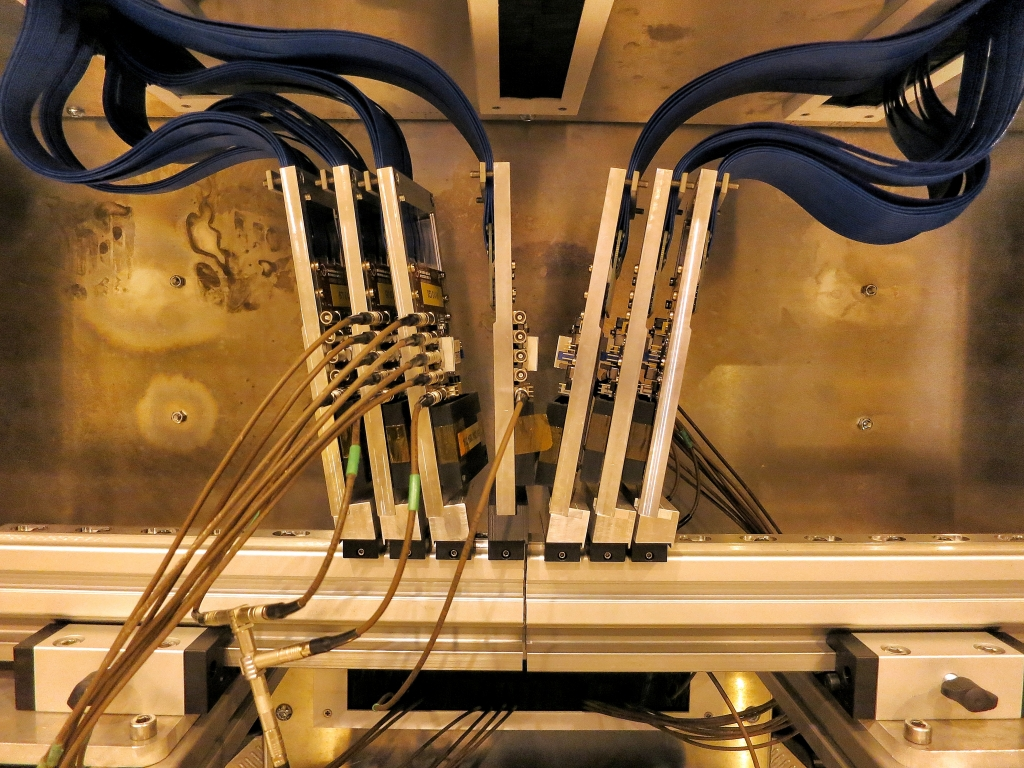
\includegraphics[width=0.6\textwidth]{ActiveEdge/Timepix3Telescope.jpeg}};
    \begin{scope}[x={(image.south east)},y={(image.north west)}]
      \node[above, color=white] at (0.5, 0.85) {Device Under Test};
      \node[above, color=white] at (0.5, 0.78) {(\textbf{DUT})};

      \draw[->, very thick, color=black](0.8, 0.25) -- (0.25, 0.25);
      \node[above, color=black] at (0.5, 0.18) {\textbf{Beam}};
      
      %% \draw[help lines,xstep=.1,ystep=.1] (0, 0) grid (1,1);
      %% \foreach \x in {0,1,...,9} { \node [anchor=north] at (\x/10,0) {0.\x}; }
      %% \foreach \y in {0,1,...,9} { \node [anchor=east] at (0,\y/10) {0.\y}; }
      
    \end{scope}
  \end{tikzpicture} 
  \caption{The Timepix3 beam reference telescope with six planes for
    the tracking and the DUT in the middle inserted perpendicular to
    the beam direction.}
  \label{fig:TPX3Telescope}
\end{figure}

The material used for the mechanical support of the sensors is
described in \cref{tab:TPX3TelescopeMaterial} with a total material
budget of $2.5\%$. For the PCB, in \textsc{Geant4}, the material
G4\_BONE\_COMPACT\_ICRU is used.

\begin{table}[htbp]
  \centering
  \caption{The mechanical support material used for the telescope planes.}
  \label{tab:TPX3TelescopeMaterial}
  \begin{tabular}{c c c}
    \toprule
    Material & Thickness [mm] & X\textsubscript{0} [mm]\\
    \midrule
    PCB (G10) & 1.6 & 164.8 \\
    Sensor cover (ABS plastic) & 2 & 406.4\\
    Cooling material for the chip (Cu) & 0.1 & 14.4 \\
    ASIC (Si) & 0.7 & 93.7 \\
    Sensor (Si) & 0.3 & 93.7 \\
    \bottomrule
  \end{tabular}
\end{table}

\subsection{Coordinates system}
A Cartesian right-handed coordinate system is chosen to describe the
geometry of the telescope. The z-direction is along the beam as shown
in \cref{fig:TPX3Telescope} and the y-direction points vertically in
the up direction.

\subsection{Data acquisition system}
The data-driven zero-suppressed mode (c.f. \cref{sec:TimepixReadout})
is used for the data acquisition of the Timepix3 readout ASICs. 

The SPIDR (Speedy PIxel Detector Readout) read-out system has been
developed by NIKHEF and CERN is used~\cite{Visser:2015bsa}. This
system is able to handle high rates of data sent by the Timepix3 ASIC
at full speed. This is achieved with Xilinx Virtex-7
FPGA~\cite{XilinxVirtex7} and a 10~Gb Ethernet link. All the particles
from the SPS spill are read out using this system.

%% --------------------------------------------- %%
\section{Reconstruction and analysis software frameworks}

The offline reconstruction of the test beam data is done using two
software frameworks. The EUTelescope software
package~\cite{Rubinskiy,EutelescopeWebsite} is used to reconstruct the
tracks from the telescope and extrapolate their positions on the
DUT. For the analysis of the DUT data, the python-based software
pyEudetanalysis is used (it can be found as a GitHub
directory~\cite{pyeudet}).

\subsection{EUTelescope}
The EUTelescope software is based on the ILCSoft
framework~\cite{Aplin:2009zz}. This latter provides the basic building
blocks such as the LCIO (Linear Collider Input Output) data model, the
geometry description toolkit GEAR and a modular application framework
for event analysis Marlin~\cite{Gaede:2006pj}.

A modular analysis and reconstruction chain can be defined using
Marlin processors. Each processor implements algorithms for specific
tasks. The input parameters for the algorithms can be configured and
loaded at runtime using \textit{steering files} in XML format. For
each event, the processors are called centrally by Marlin and this
scheme offers flexibility to the users.

EUTelescope framework, originally developed for the EUDET/AIDA pixel
beam telescope~\cite{Rubinskiy:2014kza}, provides Marlin processors
for the track reconstruction and data analysis of test beam
experiments. \cref{fig:EUTelescope_EUDET_pipeline} schematically shows
the analysis strategy in EUTelescope framework starting from the raw
data recorded during the test beam to finally particle tracks
reconstruction. Since each experiment has its own data format for the
DUT, the format converter is defined by the user. This makes the
framework more flexible for testing different chip families.

\begin{figure}[htbp]
  \centering
  \begin{tikzpicture}
    \node[anchor=south west,inner sep=0] (image) at
    (0,0){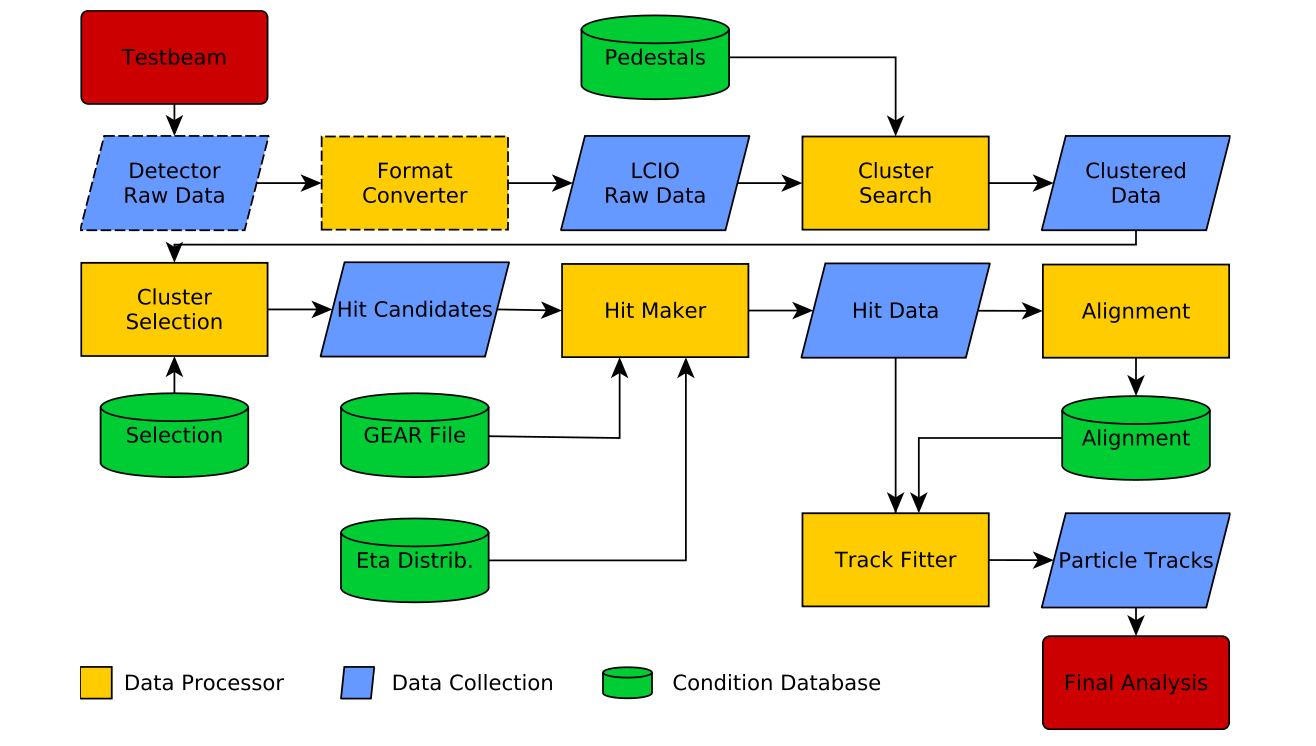
\includegraphics[width=0.8\textwidth]{figures/Telescope/EUTelescope_pipeline.png}};
    \begin{scope}[x={(image.south east)},y={(image.north west)}]
    \end{scope}
  \end{tikzpicture} 
  \caption{Data reconstruction and analysis strategy using the
    EUTelescope framework. From~\cite{Jansen:2016bkd}.}
  \label{fig:EUTelescope_EUDET_pipeline}
\end{figure}

The EUTelescope framework is adapted to be used for the data from the
Timepix3 telescope. The framework is written for a frame-based readout
mode and had to be adapted to the data-driven readout mode which was
used during the data taking. This affects mainly the definition of an
event. In a frame-based mode, an event corresponds to a frame. Whereas
in the data-driven mode, the data are written as soon as a pixel is
hit (there is no shutter). Although, in the raw file, the hits are not
ordered in time. Some pre-processing is needed to order the hits by
their time of arrival (TOA) and create events. The reconstruction
chain for the Timepix3 telescope is described in the following steps:

\begin{enumerate}
\item Converter: converts the raw files written by each telescope
planes and the DUT in a binary format to an LCIO event. The
data-driven zero-suppressed mode is used for the data acquisition of
the Timepix3 readout ASICs. This mode allows for a very low dead-time
and all the particles at the SPS spill are recorded. Every hit is
written with a 64-bit time-stamp (\texttt{long long int}) related to
the TOA (time-of-arrival). The hits written in the raw file are not
necessarily ordered in time. In the converter processor, the hits
within a timing window of 3~ms are read and filled into a vector. The
hits in the vector are ordered in time according to their time
stamps. An LCIO event is built by choosing the hits in the six
telescope planes and the DUT with time stamps differing by
$2.5\,\microsecond$. With this constraint, most probably one track per
event is obtained.
Hot pixels (with the maximum allowed frequency of 0.1) are as well
calculated and also the $\eta$-correction~\cite{Belau:1983eh} values.

\item Clustering: the clusters in each plane is found.
\item Hit making: reconstruction of the hit position for each cluster
with the $\eta$-correction method.
\item Alignment: by assuming straight tracks, the alignment processor
uses Millepede~II algorithm~\cite{Blobel20065} to align the telescope
planes with respect to each other. It consists of a least squares
minimisation problem ($\chi^2$minimisation). A proper definition of
the geometry is important.
\item Track finding: fits the tracks based on the hits on the
telescope planes with taking to account the multiple scatterings
(radiation length of the material for the described geometry),
positions of the planes. The \texttt{EUTelTestFitter} algorithm is used for the
analysis of the test-beam. (TO PUT SOME CHI2 DISTRIBUTION PLOTS). The
tracks are then extrapolated on the DUT.
\end{enumerate} 

\subsection{pyEudetAnalysis}
For the analysis of the DUT data, the python-based software
\texttt{pyEudetanalysis} is used. It can be found as a GitHub directory~\cite{pyeudet}.

%% --------------------------------------------- %%
\section{Timepix3 telescope performance}\label{sec:telescopePerformance}


\subsection{Single-hit resolution on the telescope planes}

The reconstructed hit on each telescope plane is compared to the Monte
Carlo Truth position obtained by the \textsc{Geant4}
simulations. \cref{fig:TelPlane0_MC_hit} compares the hit resolution
on the first telescope plane in x and y directions.


\begin{figure}[htbp] \centering
  \begin{subfigure}[b]{0.45\textwidth}
    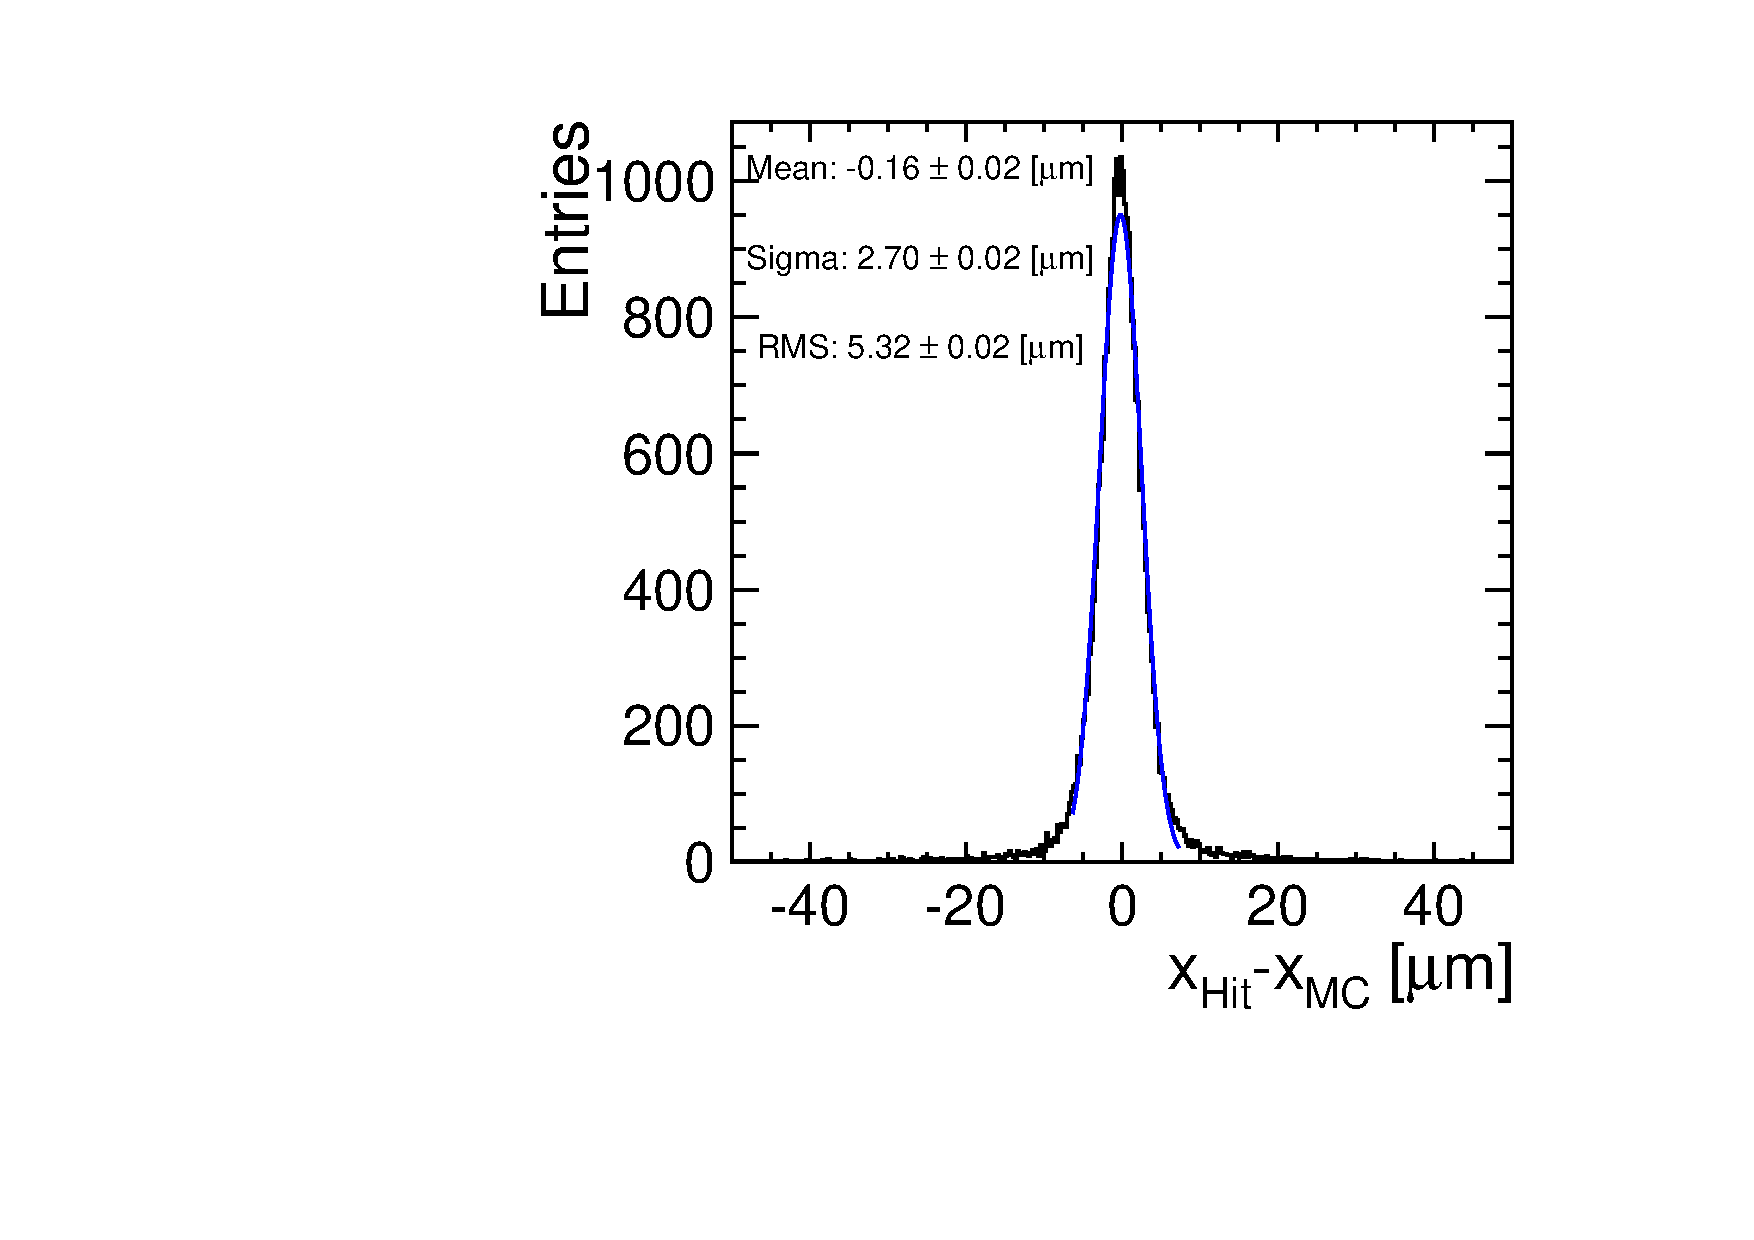
\includegraphics[width=\textwidth]{figures/Telescope/telescopePlane0_MC_vs_hit_x.pdf}
    \caption{}
  \end{subfigure}\hfill
  \begin{subfigure}[b]{0.45\textwidth}
    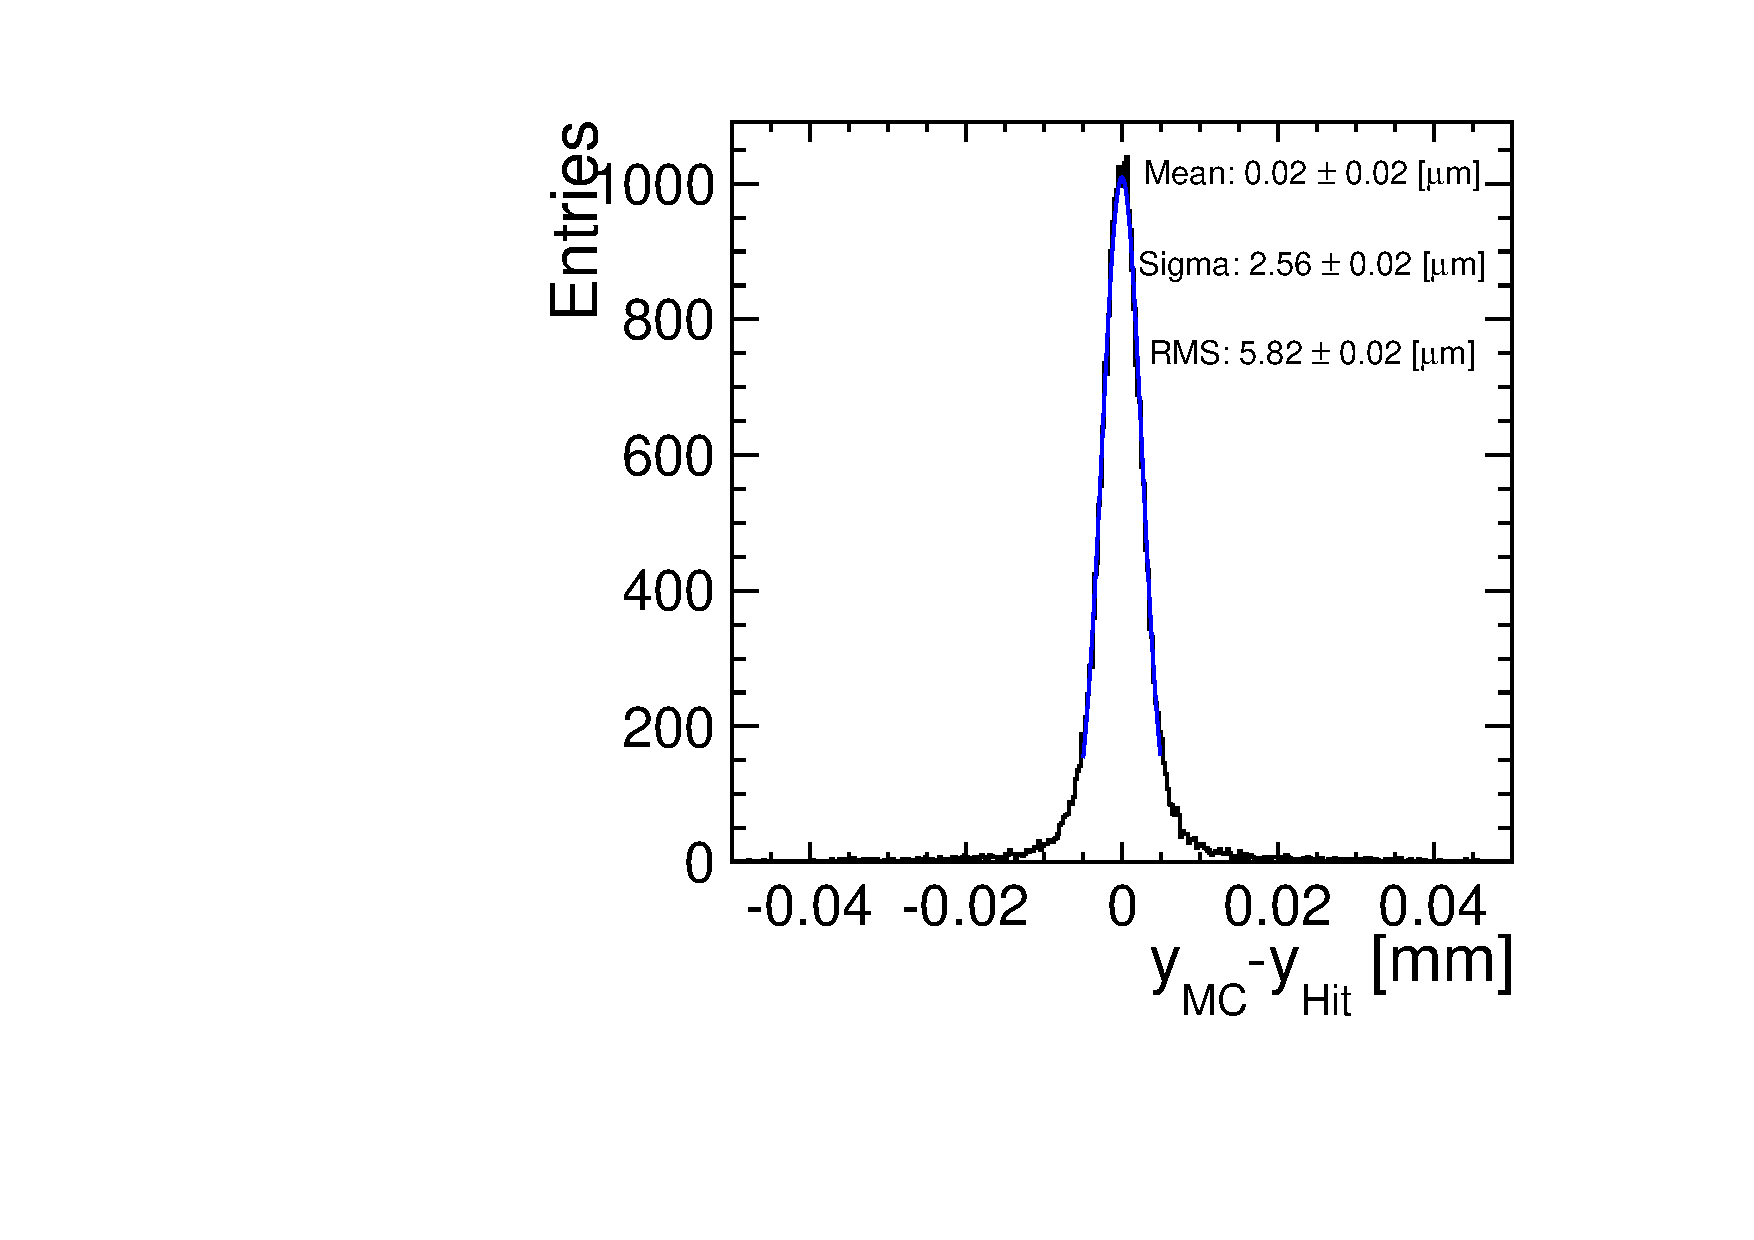
\includegraphics[width=\textwidth]{figures/Telescope/telescopePlane0_MC_vs_hit_y.pdf}
    \caption{}
  \end{subfigure}
  \caption{MC hit vs. reconstructed hit position.}
  \label{fig:TelPlane0_MC_hit}
\end{figure}

The residuals as a function of the x\textsubscript{MC} and
y\textsubscript{MC} are shown in \cref{fig:TelPlane0_MC_hit_2D}.

\begin{figure}[htbp] \centering
  \begin{subfigure}[b]{0.45\textwidth}
    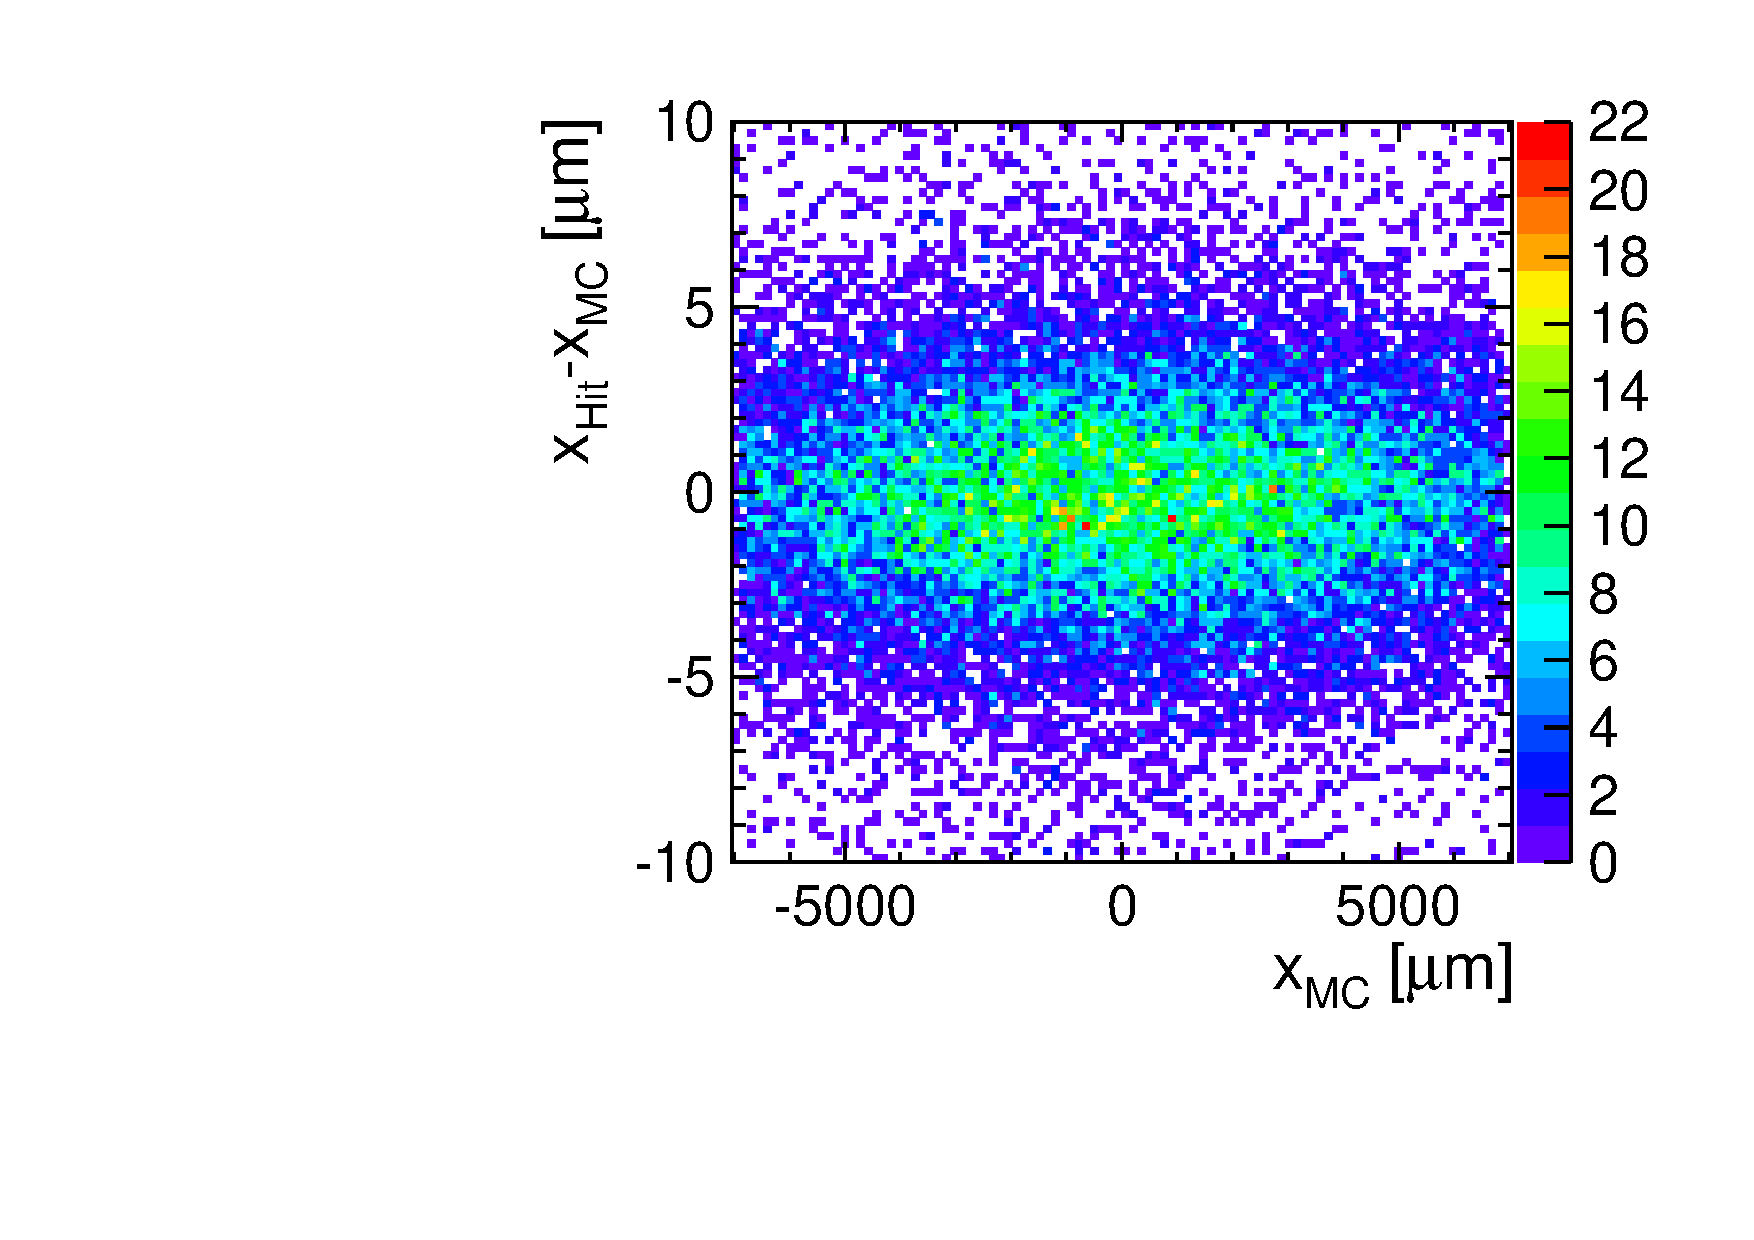
\includegraphics[width=\textwidth]{figures/Telescope/telescopePlane0_MC_vs_hit_x_2D.pdf}
    \caption{}
  \end{subfigure}\hfill
  \begin{subfigure}[b]{0.45\textwidth}
    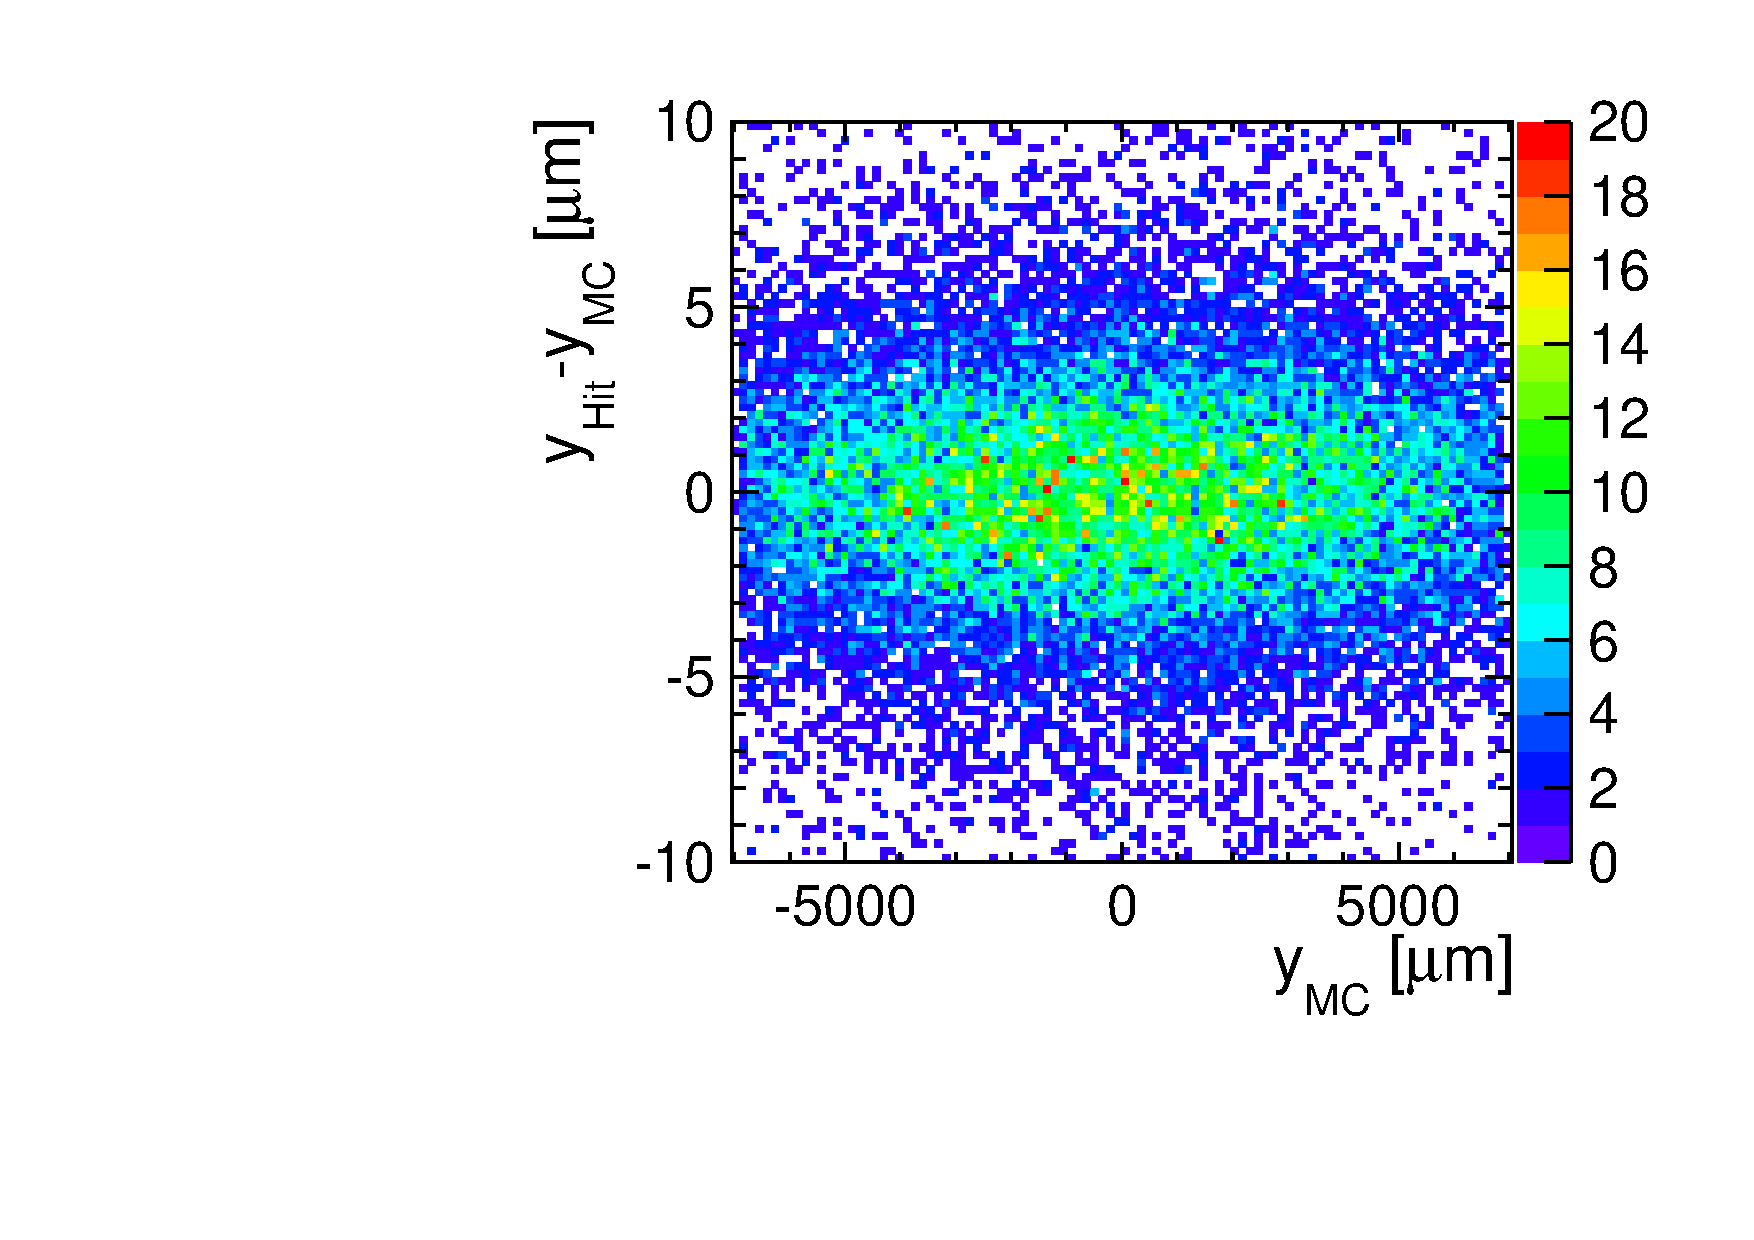
\includegraphics[width=\textwidth]{figures/Telescope/telescopePlane0_MC_vs_hit_y_2D.pdf}
    \caption{}
  \end{subfigure}
  \caption{MC hit vs. reconstructed hit position.}
  \label{fig:TelPlane0_MC_hit_2D}
\end{figure}


The tracking resolution on the DUT ($100\,\micron$ thick sensor) in
the x and y directions is shown in \cref{fig:DUT_MC_track}.
\begin{figure}[htbp] \centering
  \begin{subfigure}[b]{0.45\textwidth}
    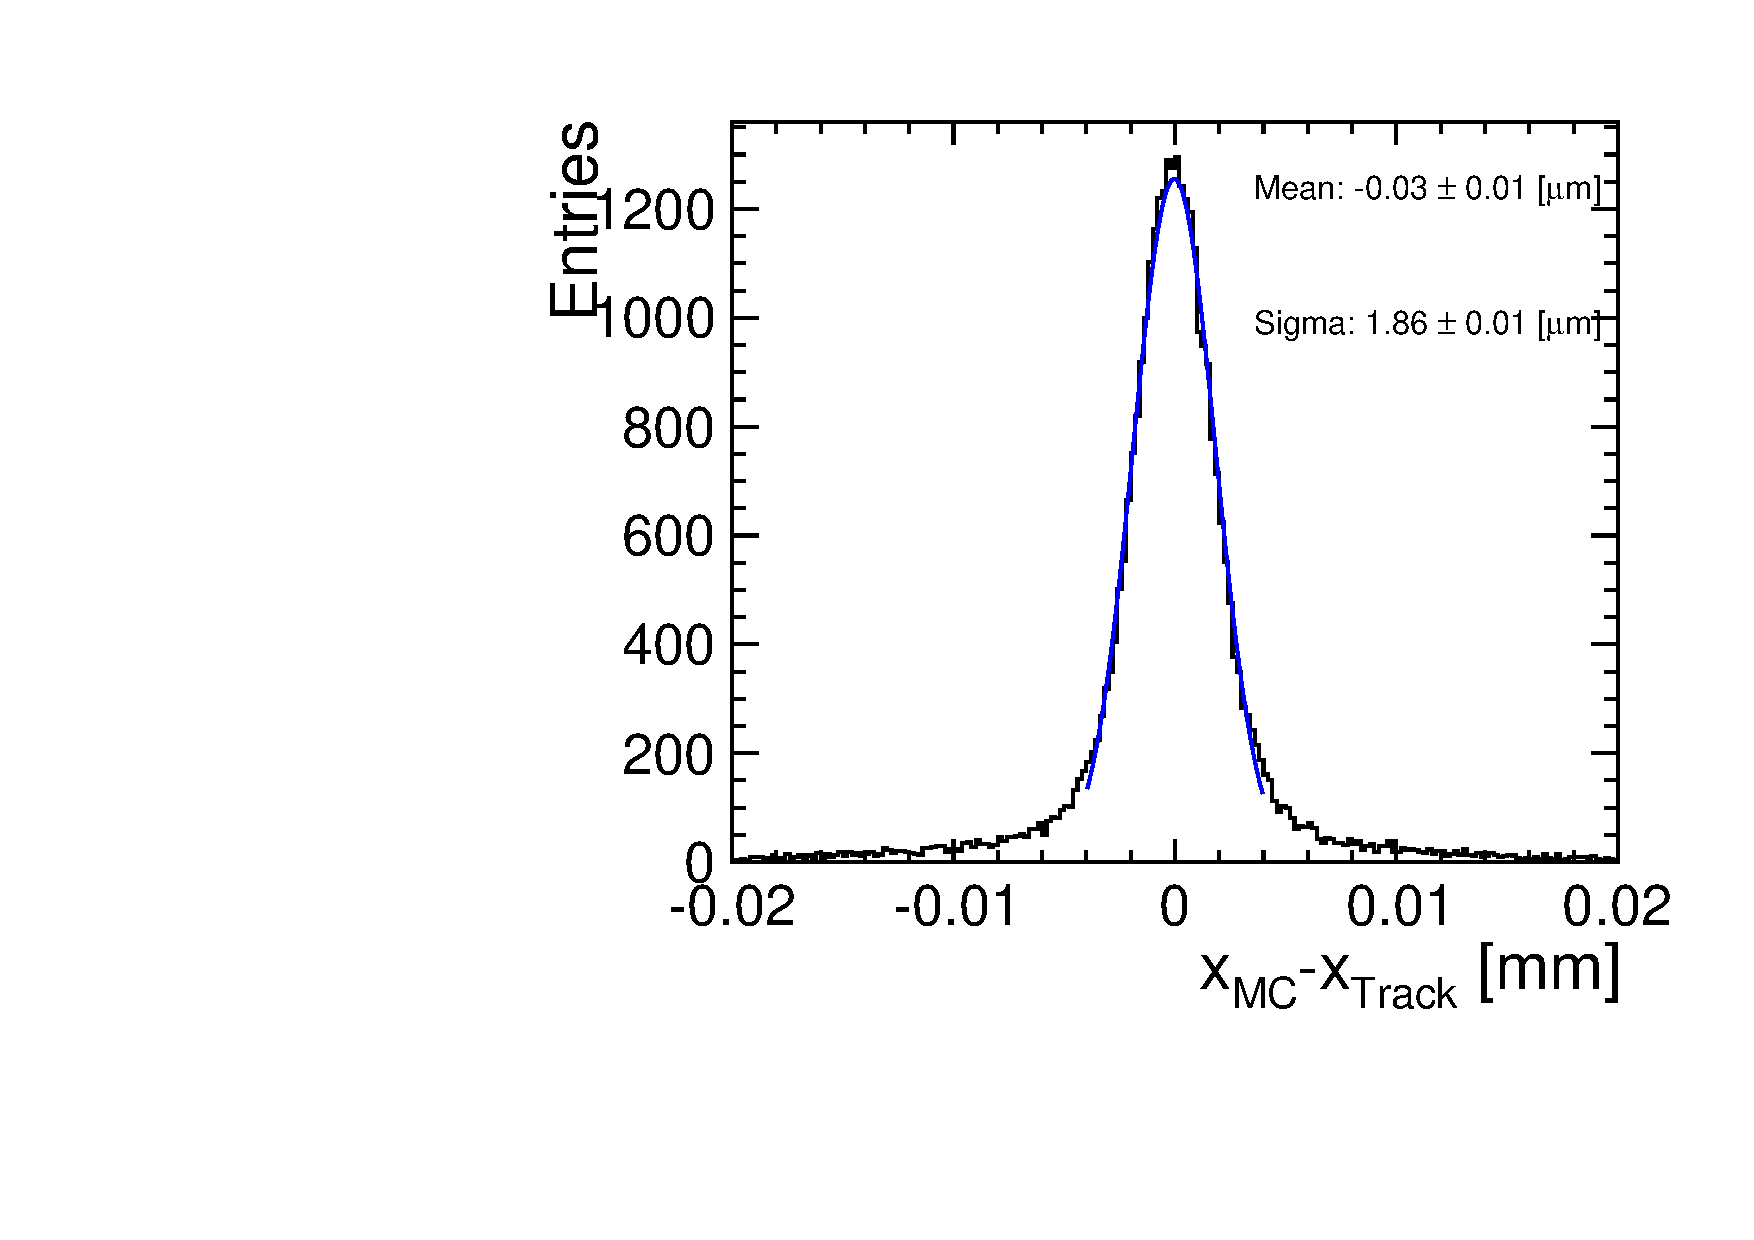
\includegraphics[width=\textwidth]{figures/Telescope/Unbiased_trackRes_DUT_x.pdf}
    \caption{}
  \end{subfigure}\hfill
  \begin{subfigure}[b]{0.45\textwidth}
    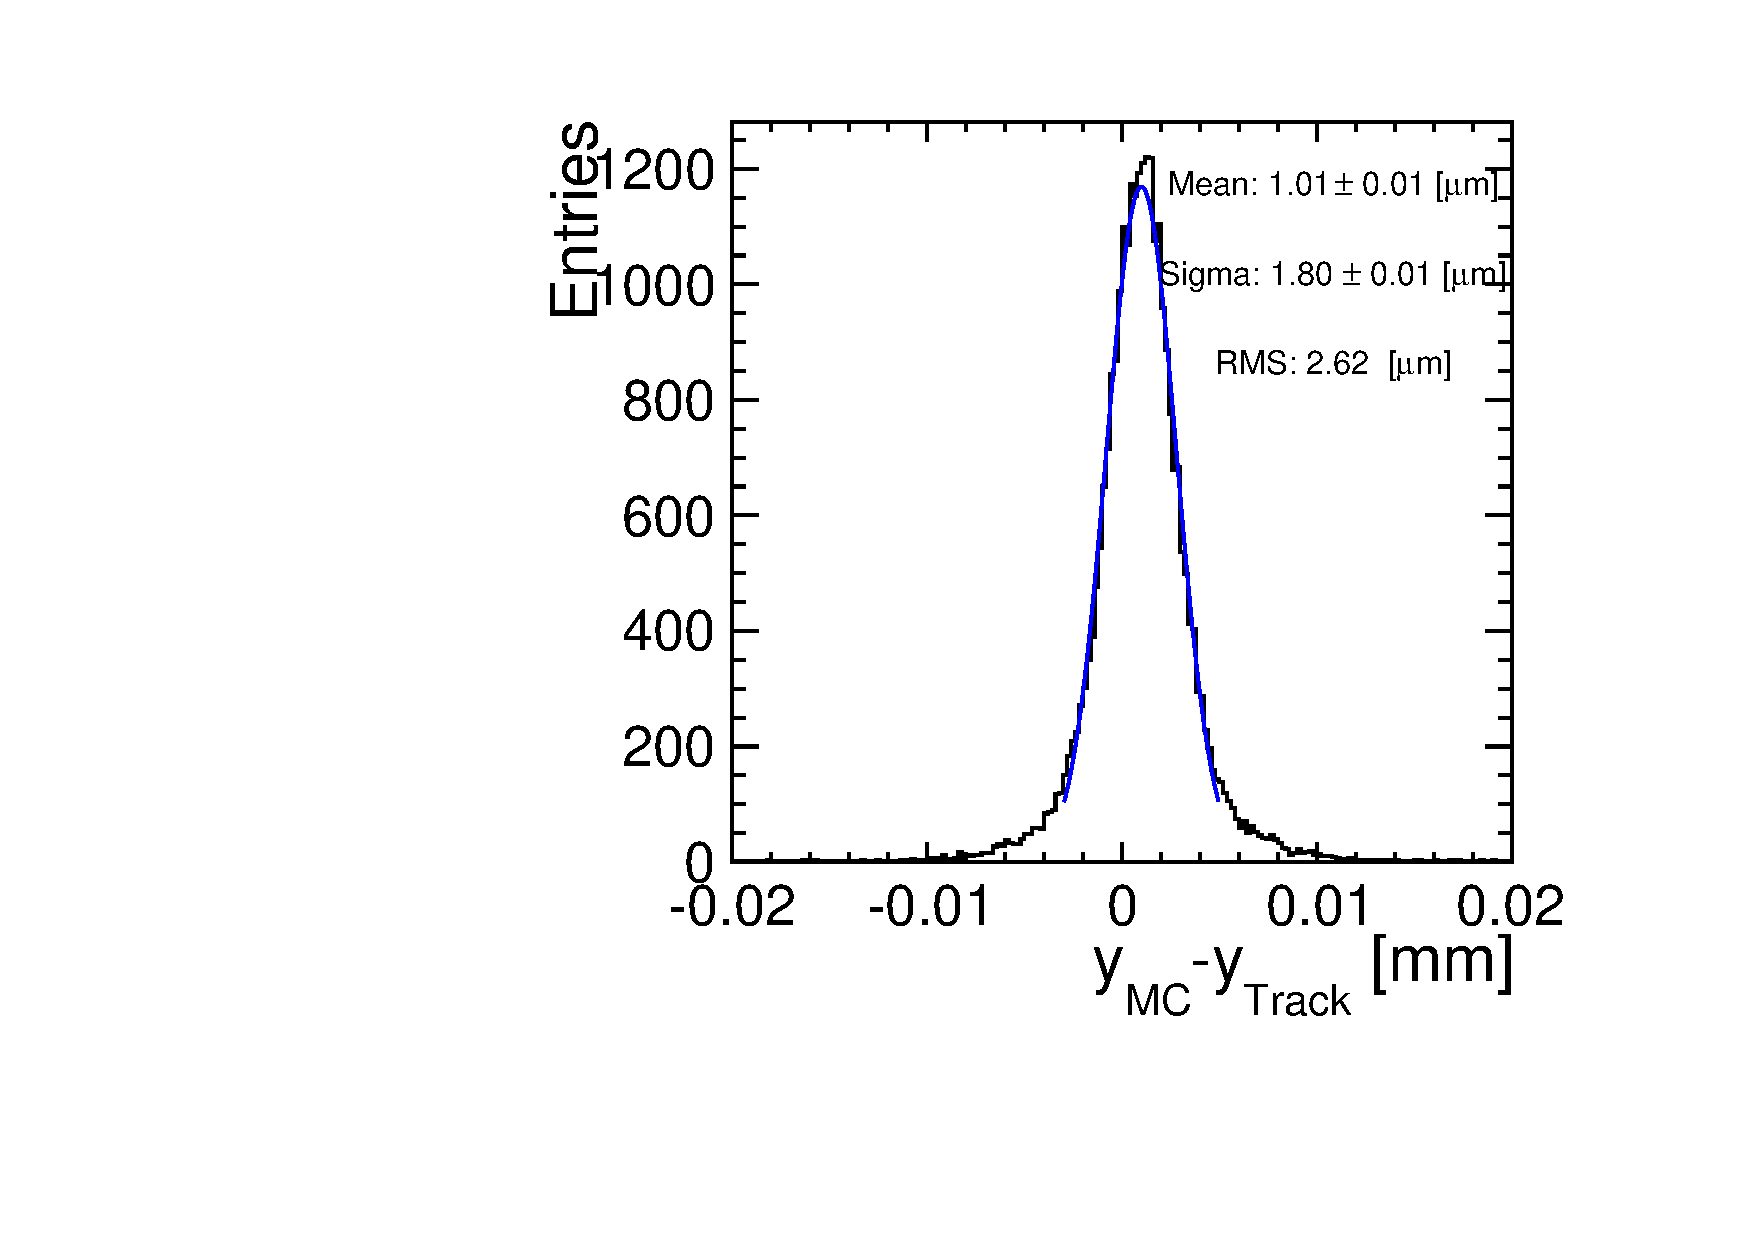
\includegraphics[width=\textwidth]{figures/Telescope/Unbiased_trackRes_DUT_y.pdf}
    \caption{}
  \end{subfigure}
  \caption{The tracking resolution on the DUT comparing the
    reconstructed track position to the true position of the particles
    coming from \textsc{Geant4}.}
  \label{fig:DUT_MC_track}
\end{figure}


In 2D the tracking resolution on the DUT is shown in \cref{fig:DUT_MC_track_2D}.
\begin{figure}[htbp] \centering
  \begin{subfigure}[b]{0.45\textwidth}
    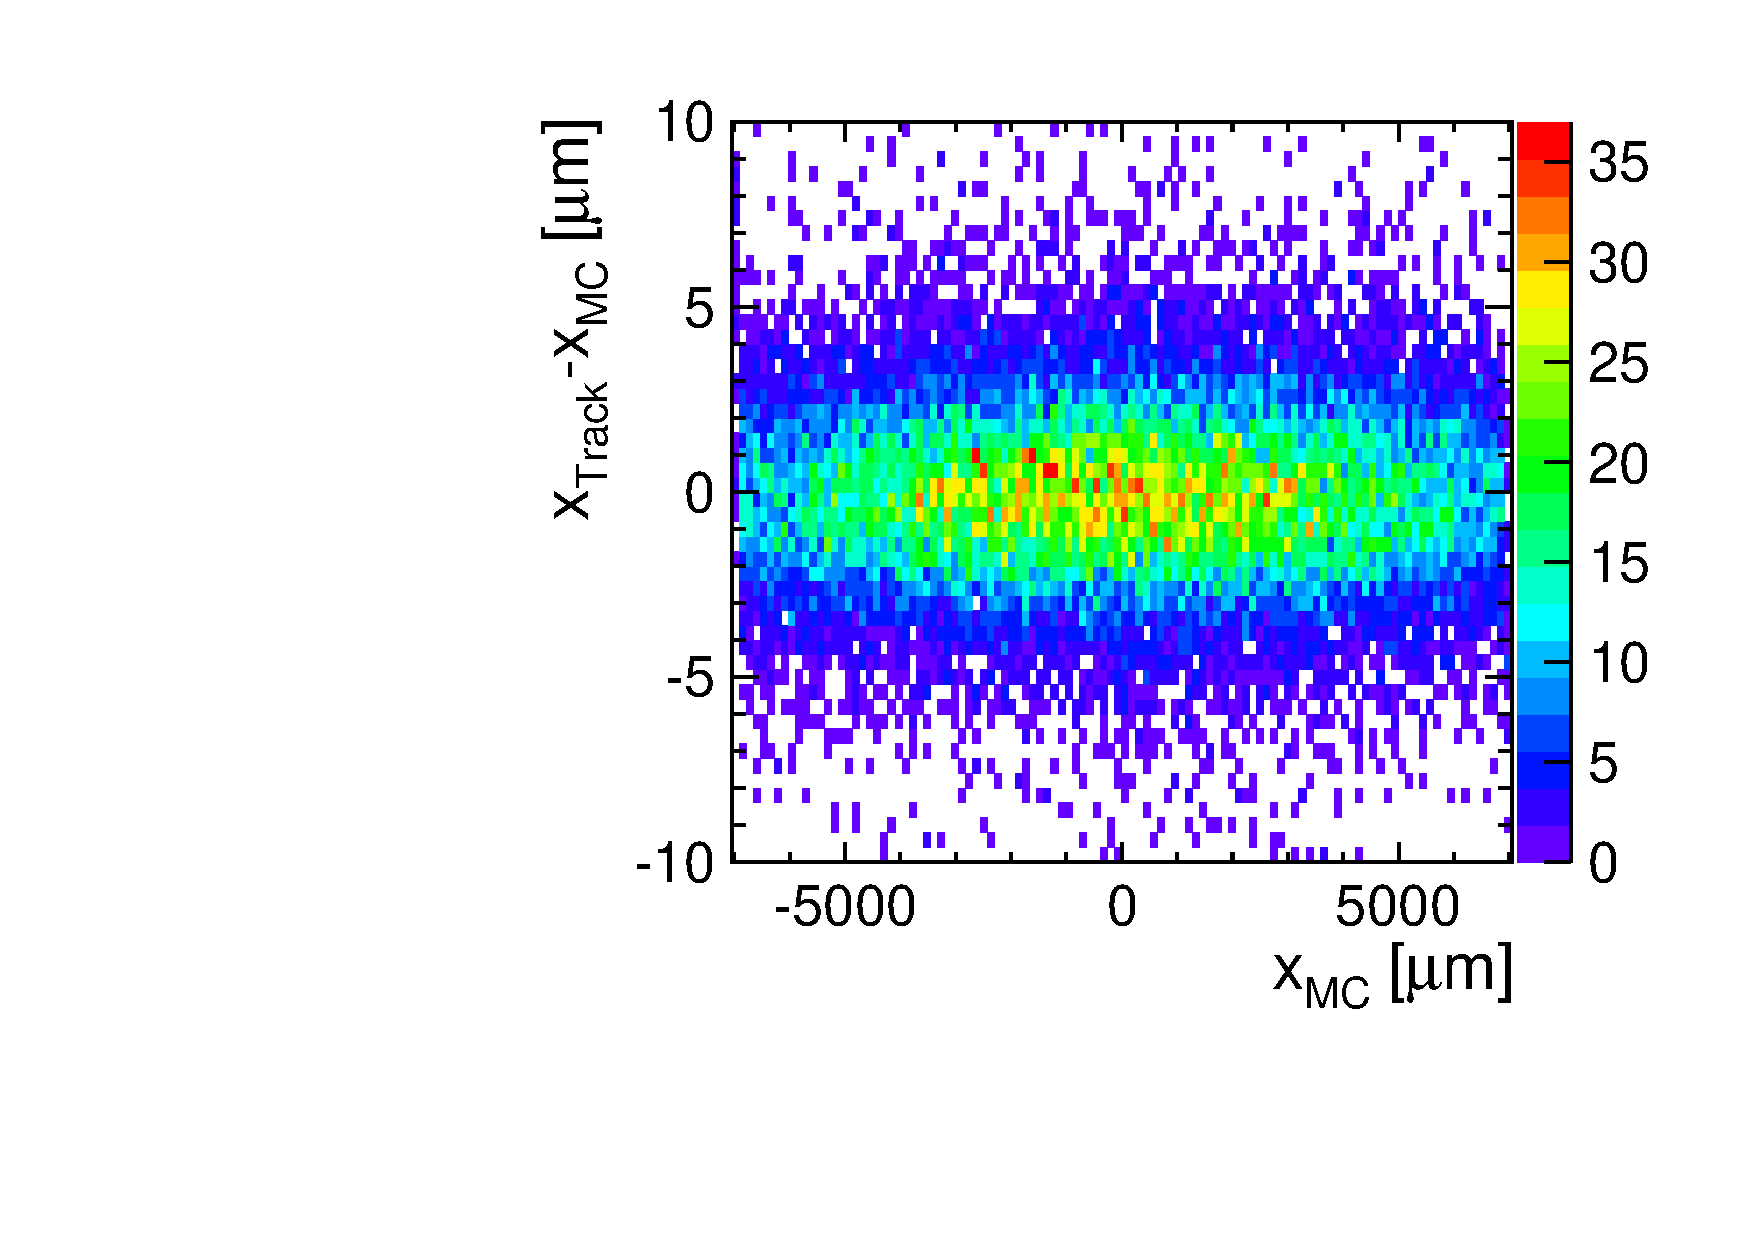
\includegraphics[width=\textwidth]{figures/Telescope/Unbiased_trackRes_DUT_x_2D.pdf}
    \caption{}
  \end{subfigure}\hfill
  \begin{subfigure}[b]{0.45\textwidth}
    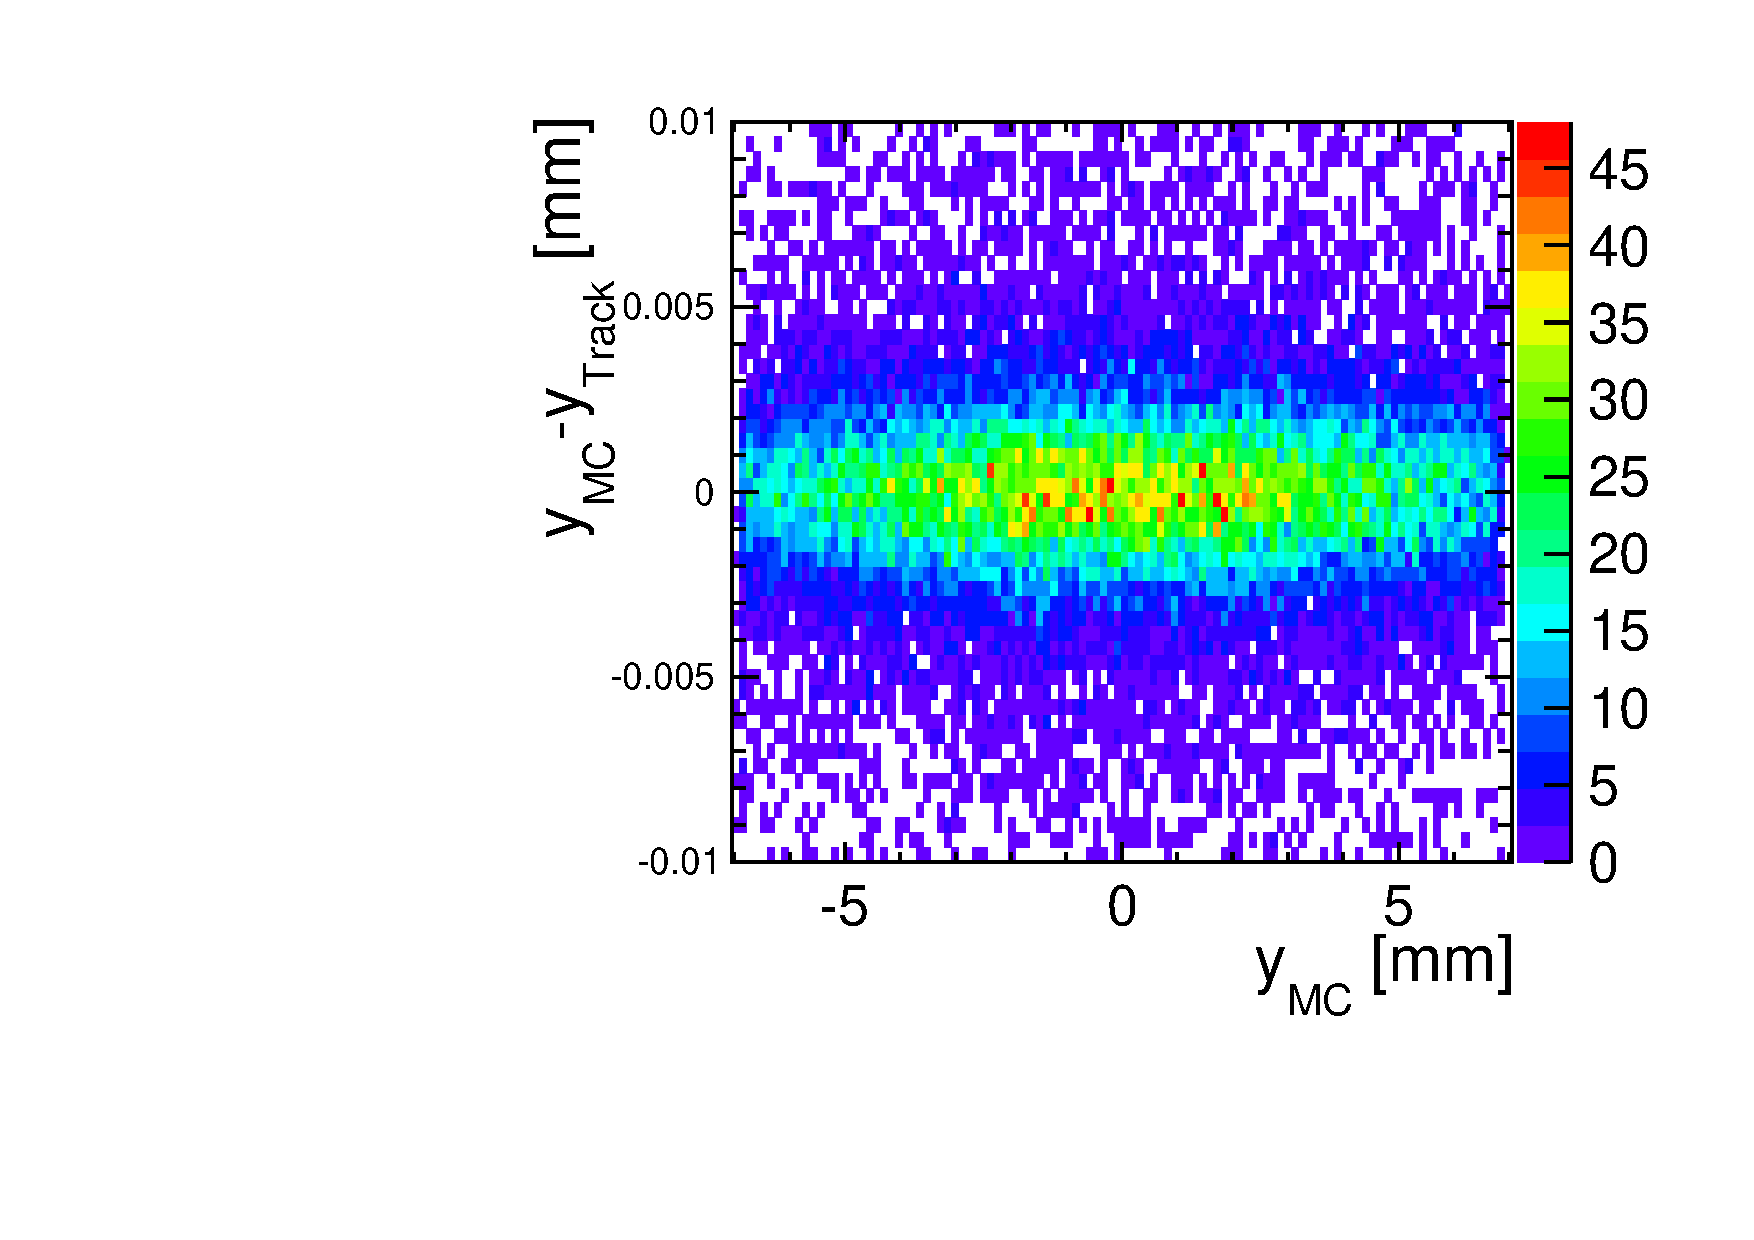
\includegraphics[width=\textwidth]{figures/Telescope/Unbiased_trackRes_DUT_y_2D.pdf}
    \caption{}
  \end{subfigure}
  \caption{Track vs. MC position on the DUT.}
  \label{fig:DUT_MC_track_2D}
\end{figure}

\subsection{Biased residuals on each telescope plane}

In simulation the material for the PCB in simulations is chosen to be
an epoxy (G4\_PLEXIGLASS) with a density of 1.19~g~\inversecmcubic and
a radiation length of X\textsubscript{0}=4.06~g~\inversecmsquared
(3.41~cm).


The cluster size distribution and the collected charge comparing data
and simulations is shown in \cref{fig:TelescopeCluSize_data_simu}.

\begin{figure}[htbp] \centering
  \begin{subfigure}[b]{0.3\textwidth}
    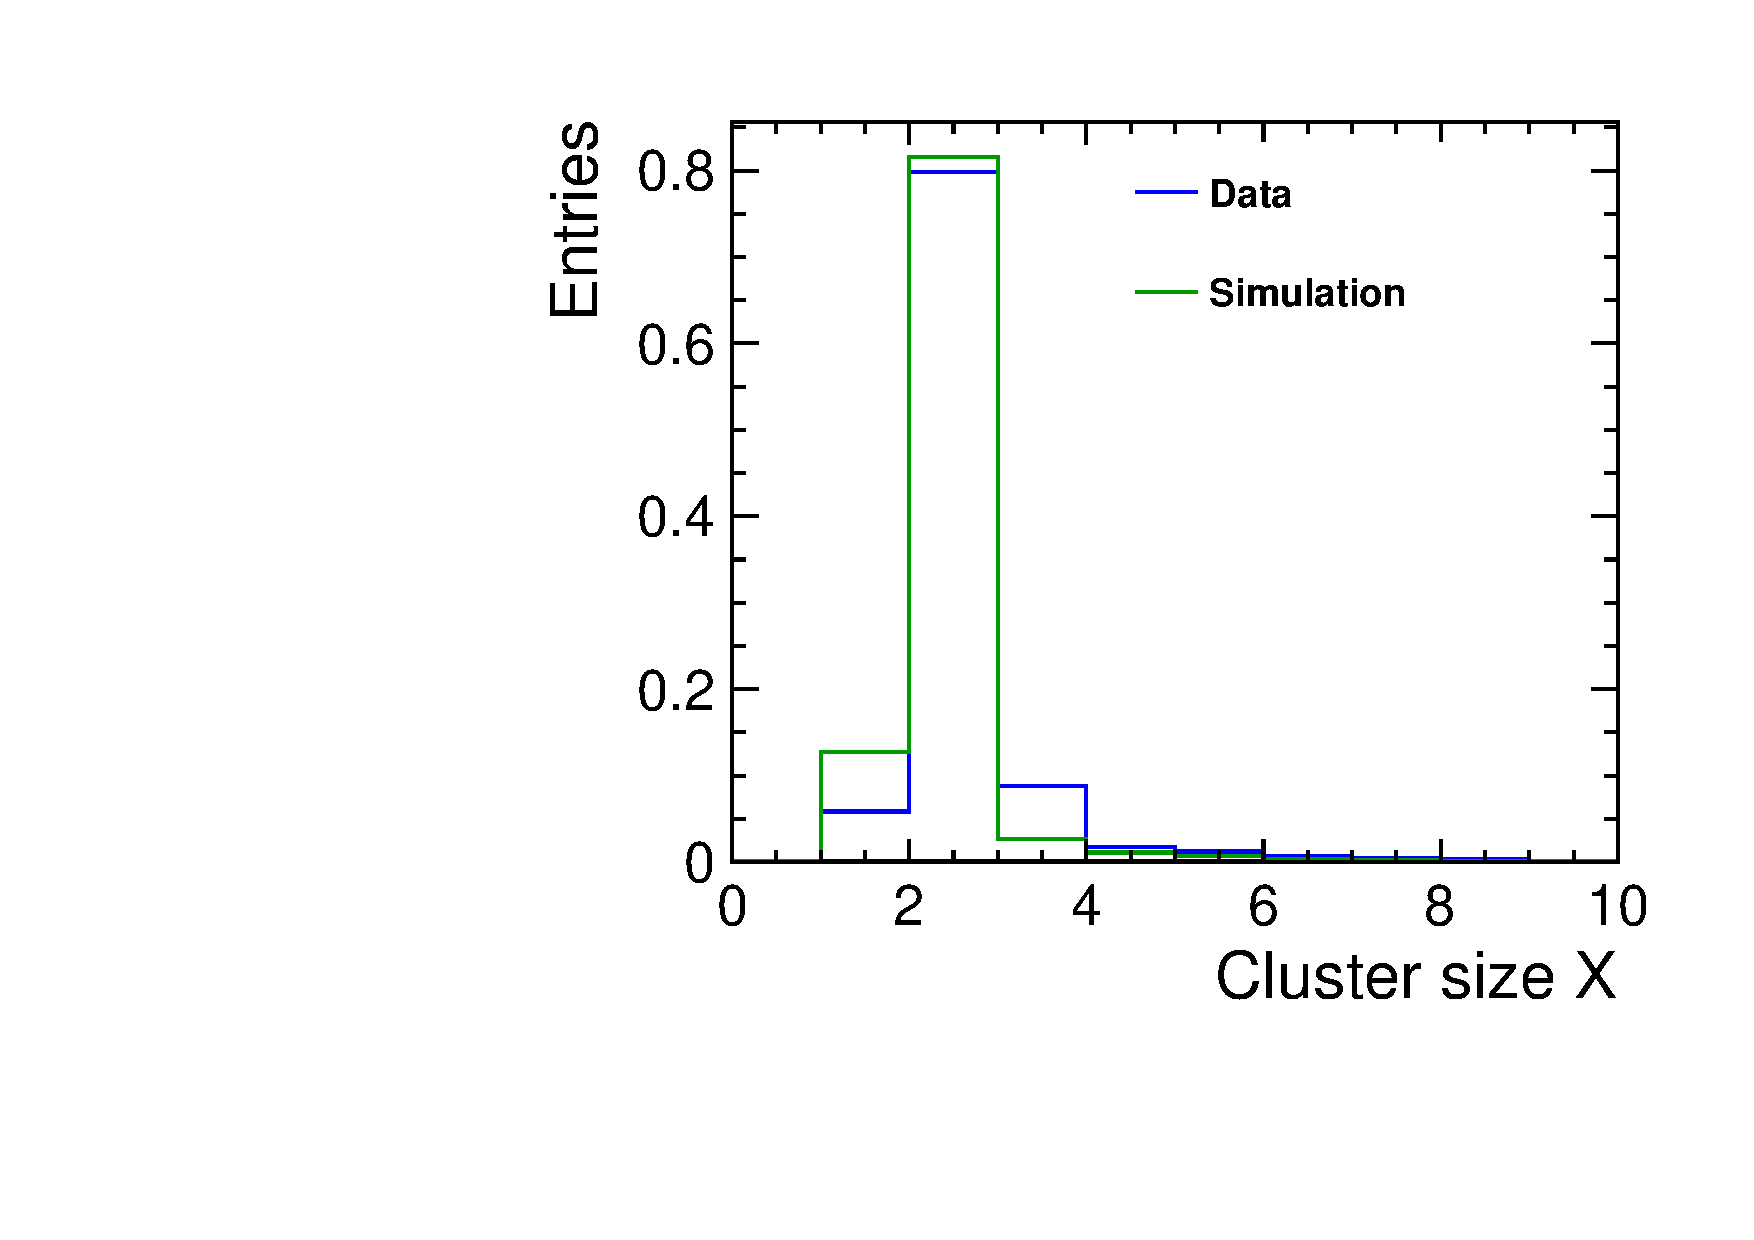
\includegraphics[width=\textwidth]{figures/Telescope/biasedResiduals/clusterSizeX_telescope0_data_simu.pdf}
    \caption{}
  \end{subfigure}\hfill
  \begin{subfigure}[b]{0.3\textwidth}
    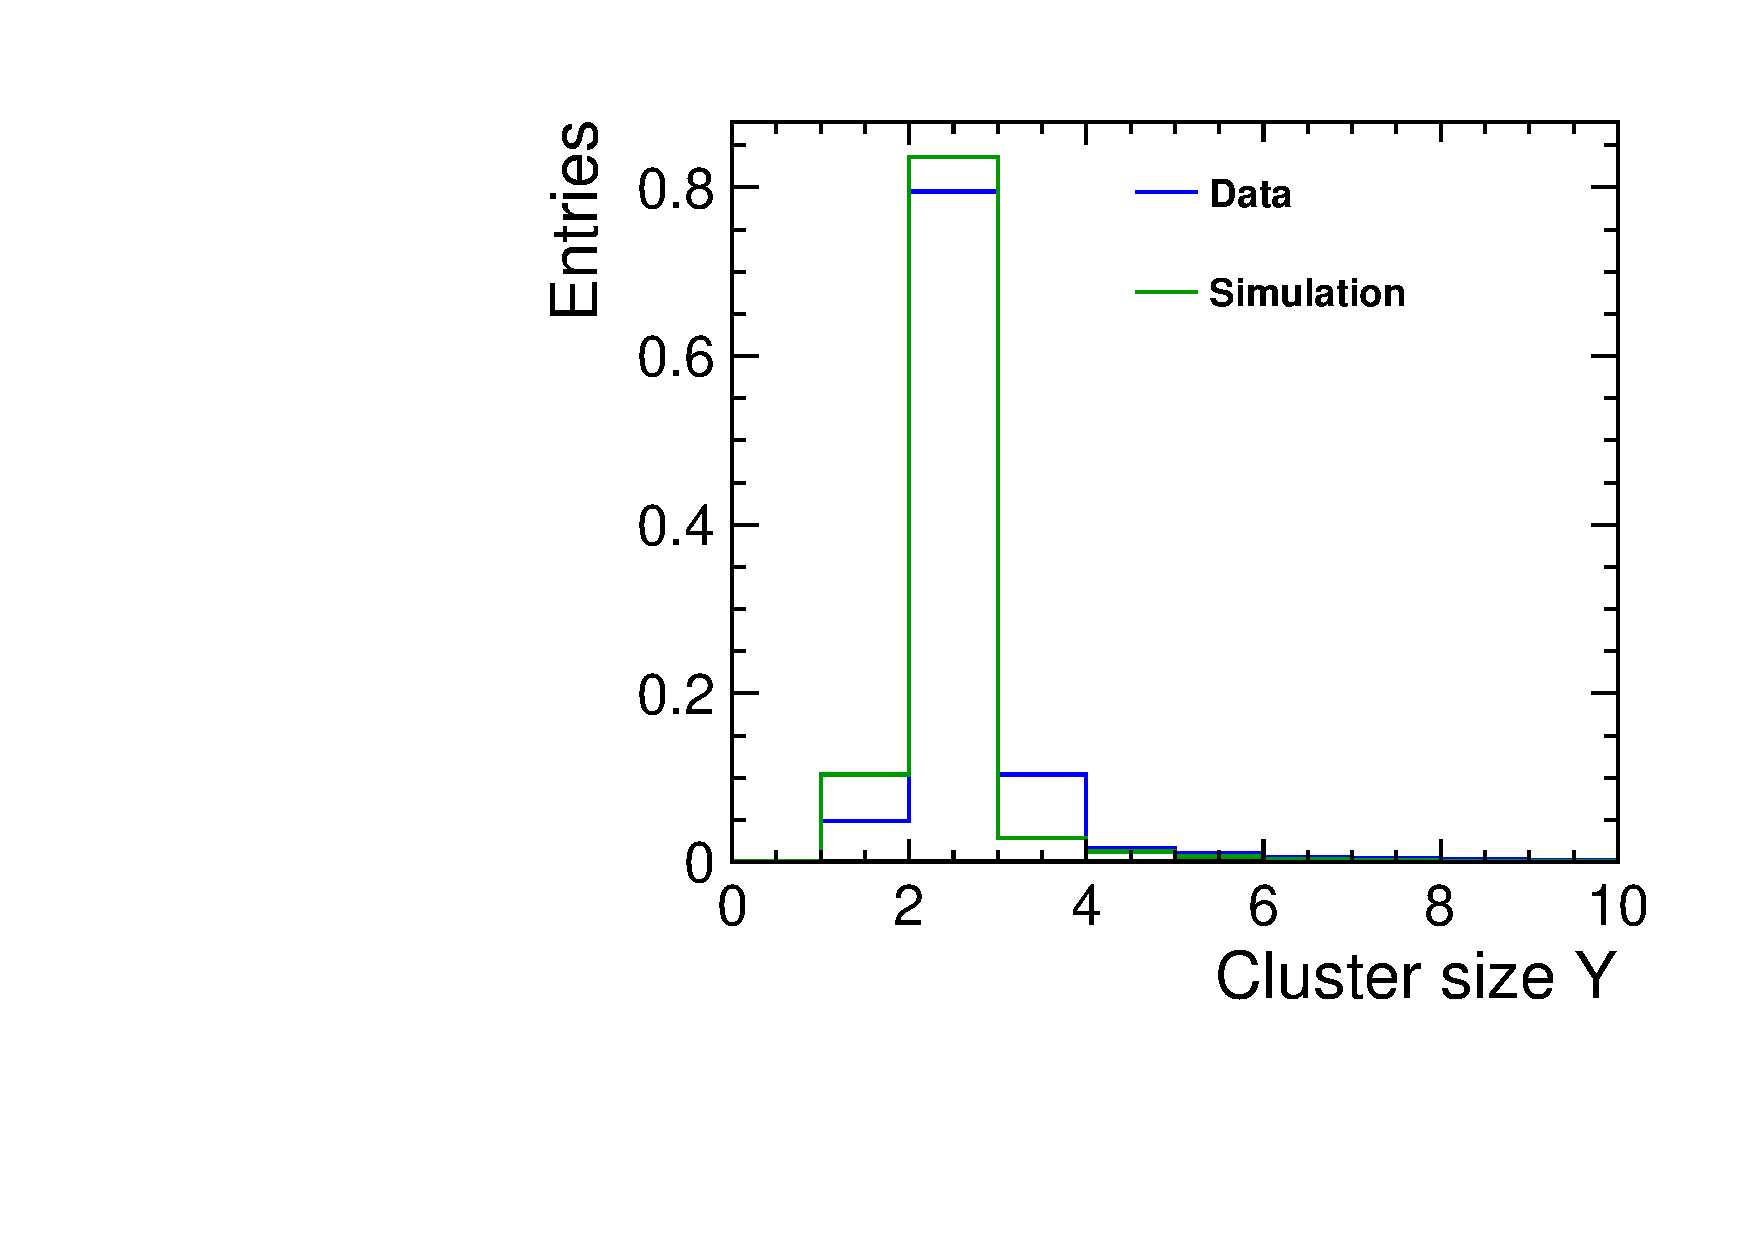
\includegraphics[width=\textwidth]{figures/Telescope/biasedResiduals/clusterSizeY_telescope0_data_simu.pdf}
    \caption{}
  \end{subfigure}\hfill
  \begin{subfigure}[b]{0.3\textwidth}
    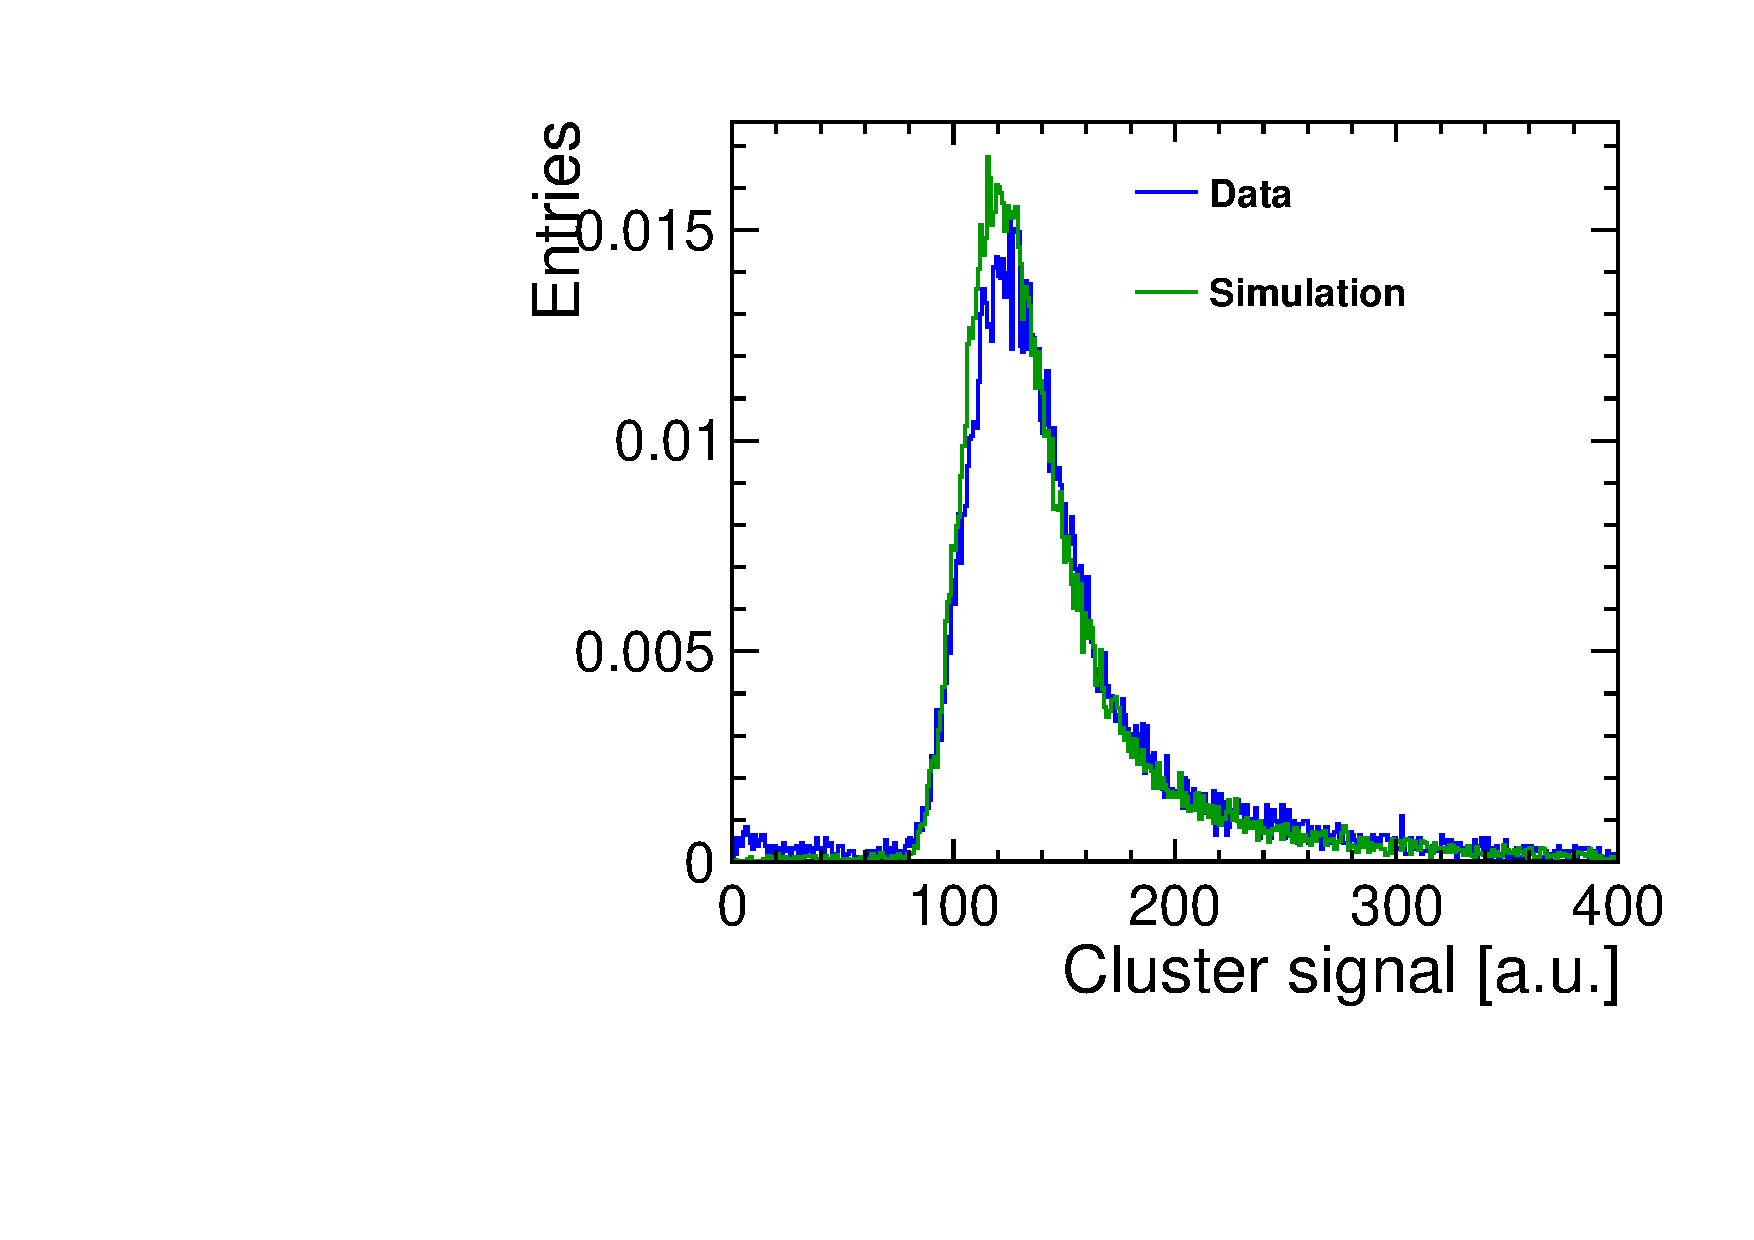
\includegraphics[width=\textwidth]{figures/Telescope/biasedResiduals/clusterSignal_telescope0_data_simu.pdf}
    \caption{}
  \end{subfigure}
  \caption{data run 661, simulation run 54.}
  \label{fig:TelescopeCluSize_data_simu}
\end{figure}

The biased residuals (RMS) comparing data and simulation in
\cref{fig:telescopeBiasedRMS_data_simu} (the distributions are given
in
\cref{fig:telescope_biasedResiduals_data_X,fig:telescope_biasedResiduals_data_Y}
for data and
\cref{fig:telescope_biasedResiduals_simu_X,fig:telescope_biasedResiduals_simu_Y}
for simulation.
\begin{figure}[htbp] \centering
  \begin{subfigure}[b]{0.45\textwidth}
    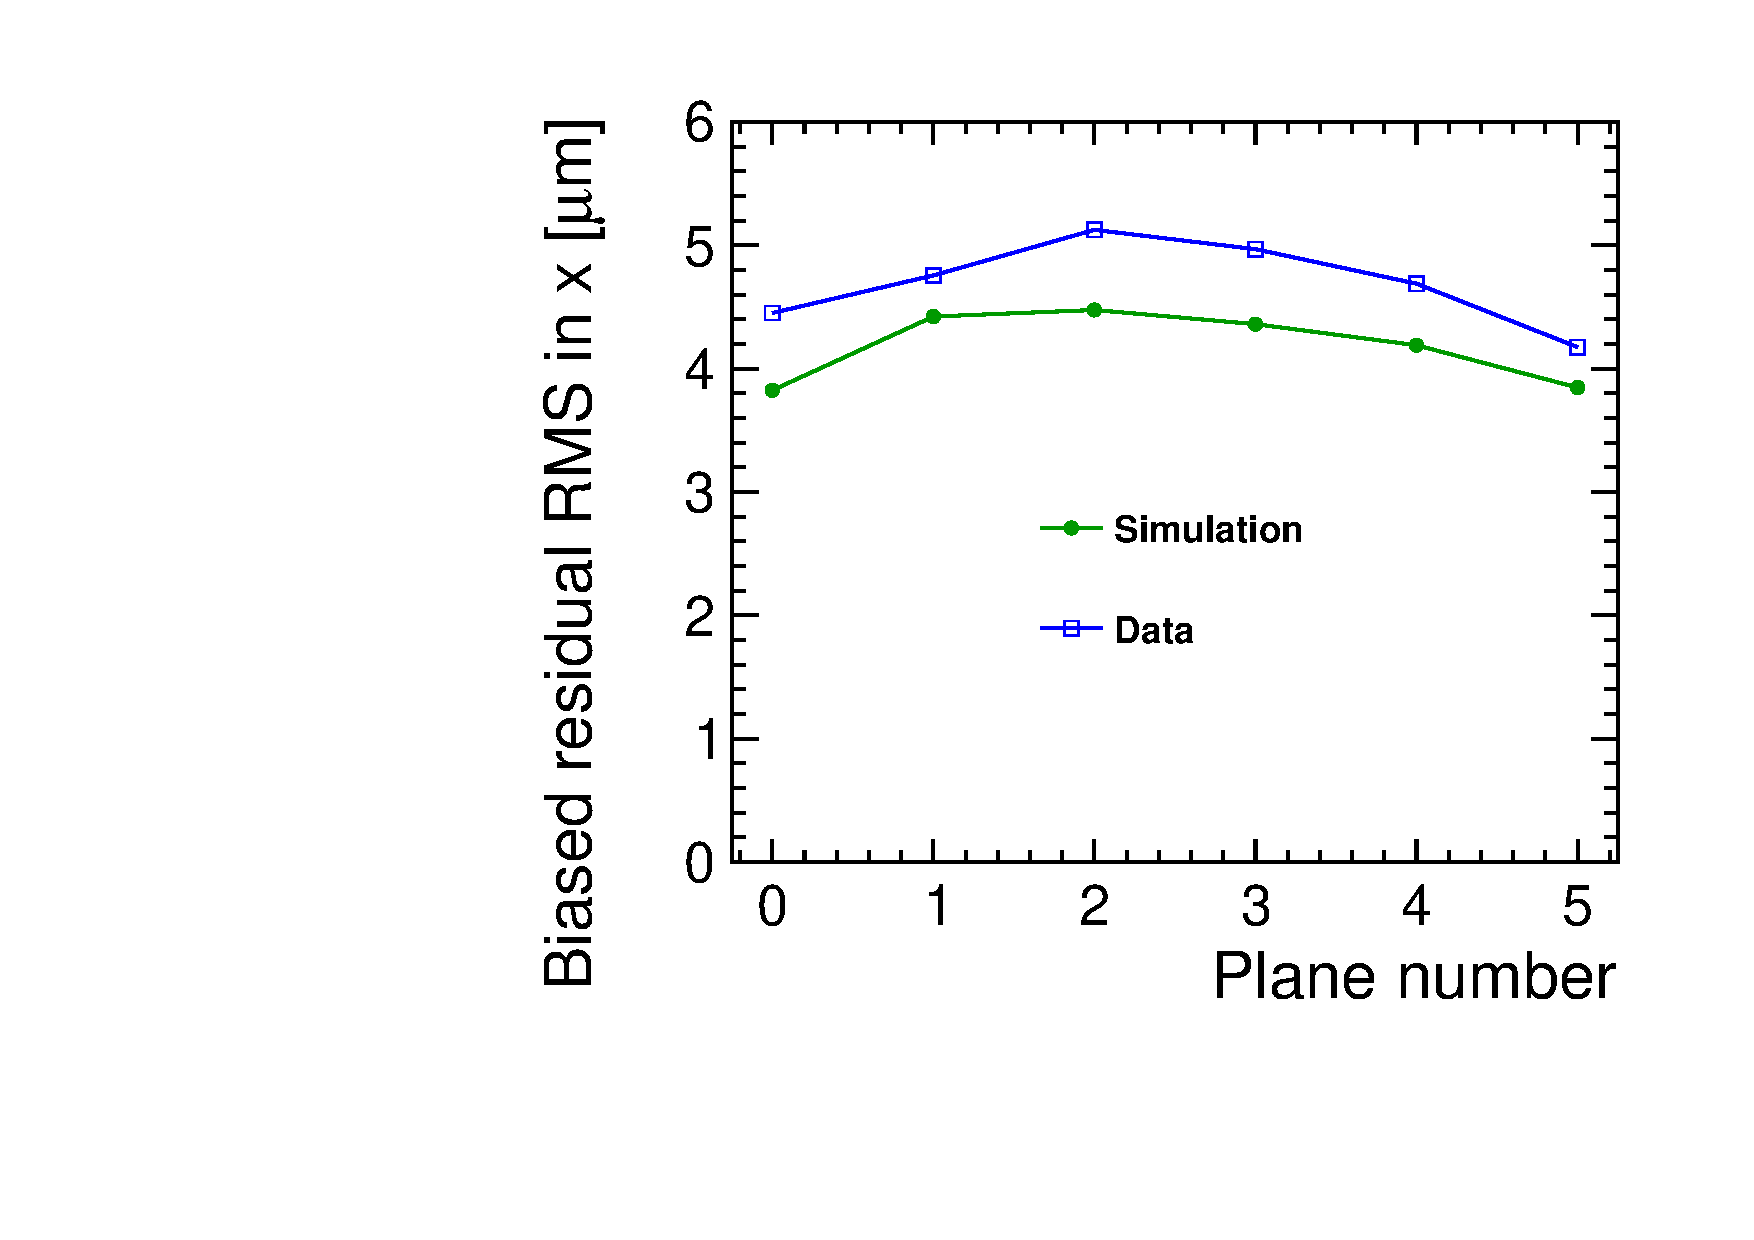
\includegraphics[width=\textwidth]{figures/Telescope/biasedResiduals/RMSX_simu_vs_data.pdf}
    \caption{}
  \end{subfigure}\hfill
  \begin{subfigure}[b]{0.45\textwidth}
    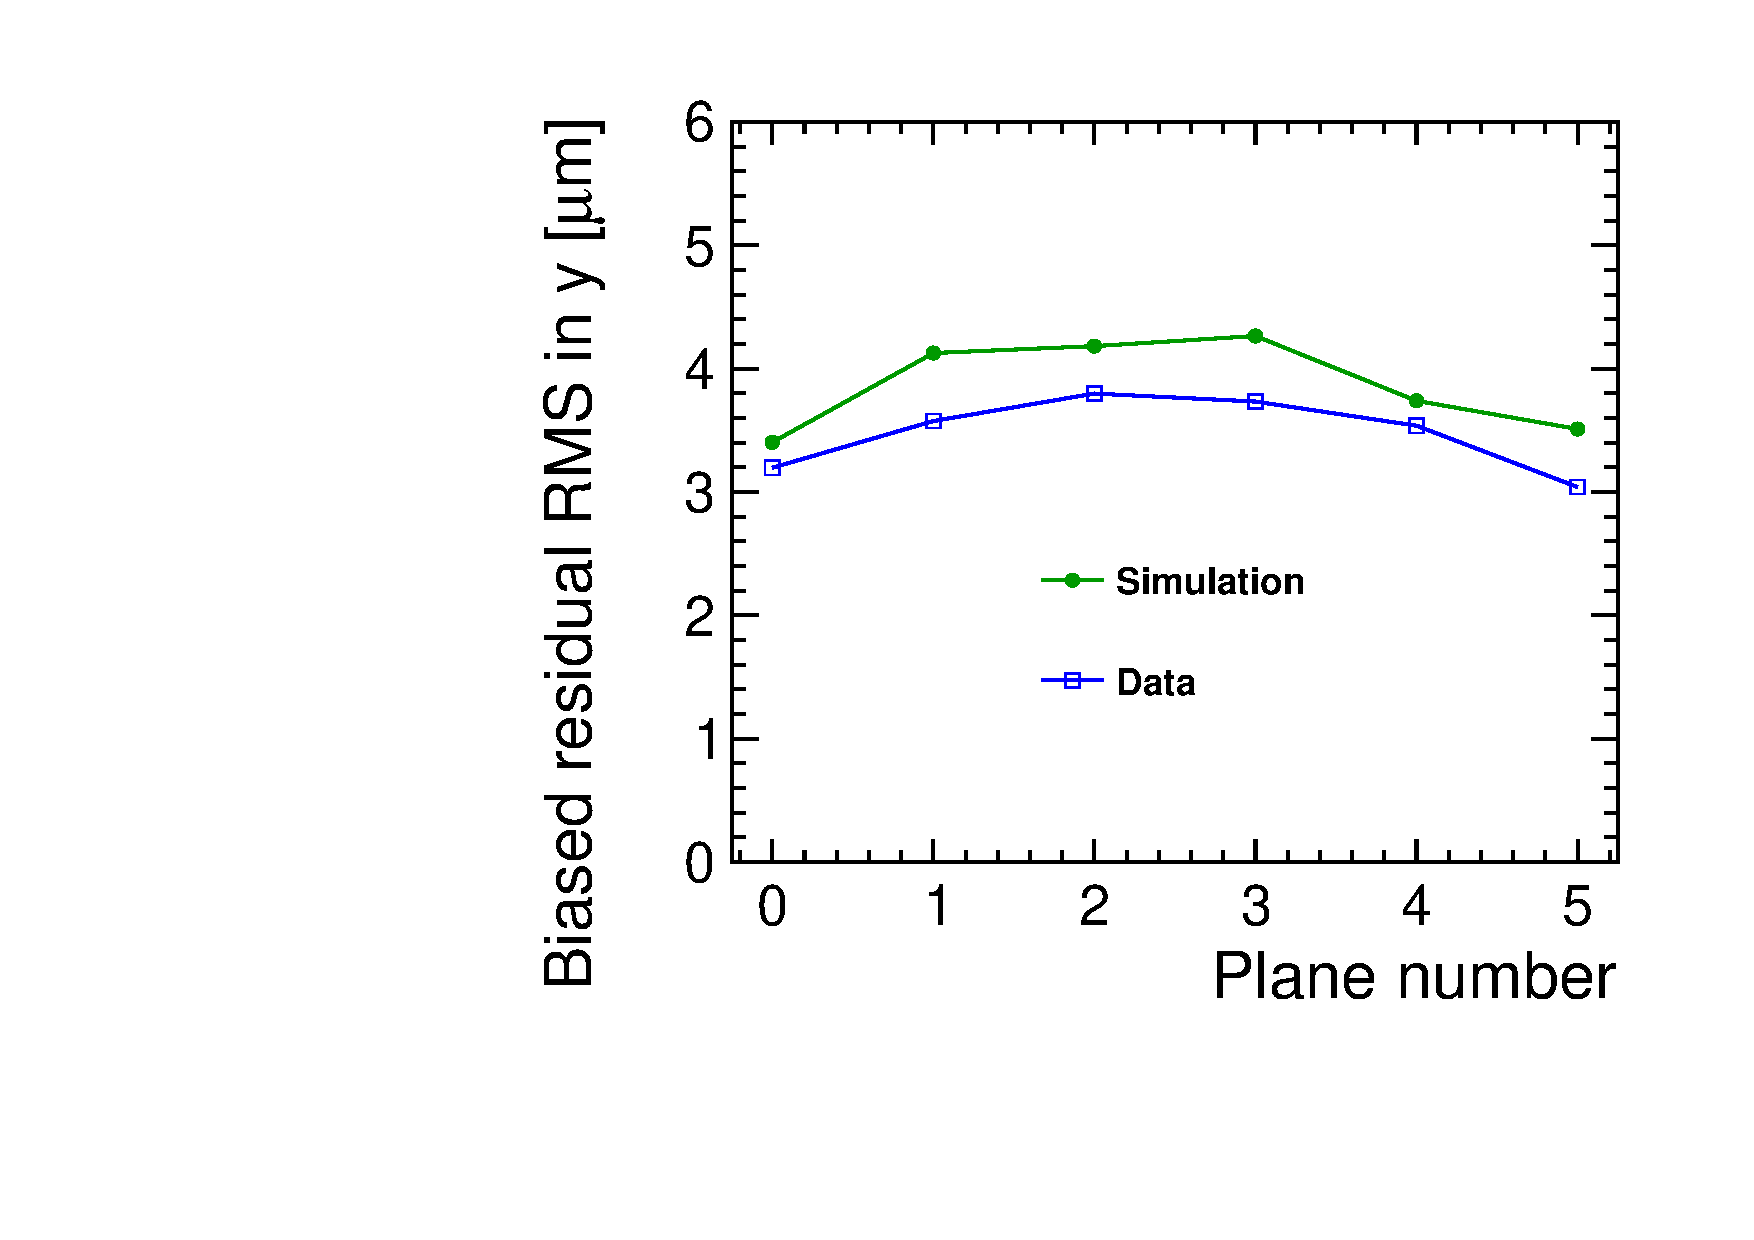
\includegraphics[width=\textwidth]{figures/Telescope/biasedResiduals/RMSY_simu_vs_data.pdf}
    \caption{}
  \end{subfigure}
  \caption{data run 661, simulation run 54.}
  \label{fig:telescopeBiasedRMS_data_simu}
\end{figure}

%% --------------------------------------------- %%

\subsection{Beam angle}

For MC beam angle distribution:

\begin{equation}
  \phi=arctan{{x_2-x_{DUT}} \over {z_2-z_{DUT}}} \; ,
  \label{eq:beamAnglePhi}
\end{equation}

\begin{equation}
  \theta=arctan{{y_2-y_{DUT}} \over {z_2-z_{DUT}}} \; ,
  \label{eq:beamAngleTheta}
\end{equation}

\begin{figure}[htbp] \centering
  \begin{subfigure}[b]{0.45\textwidth}
    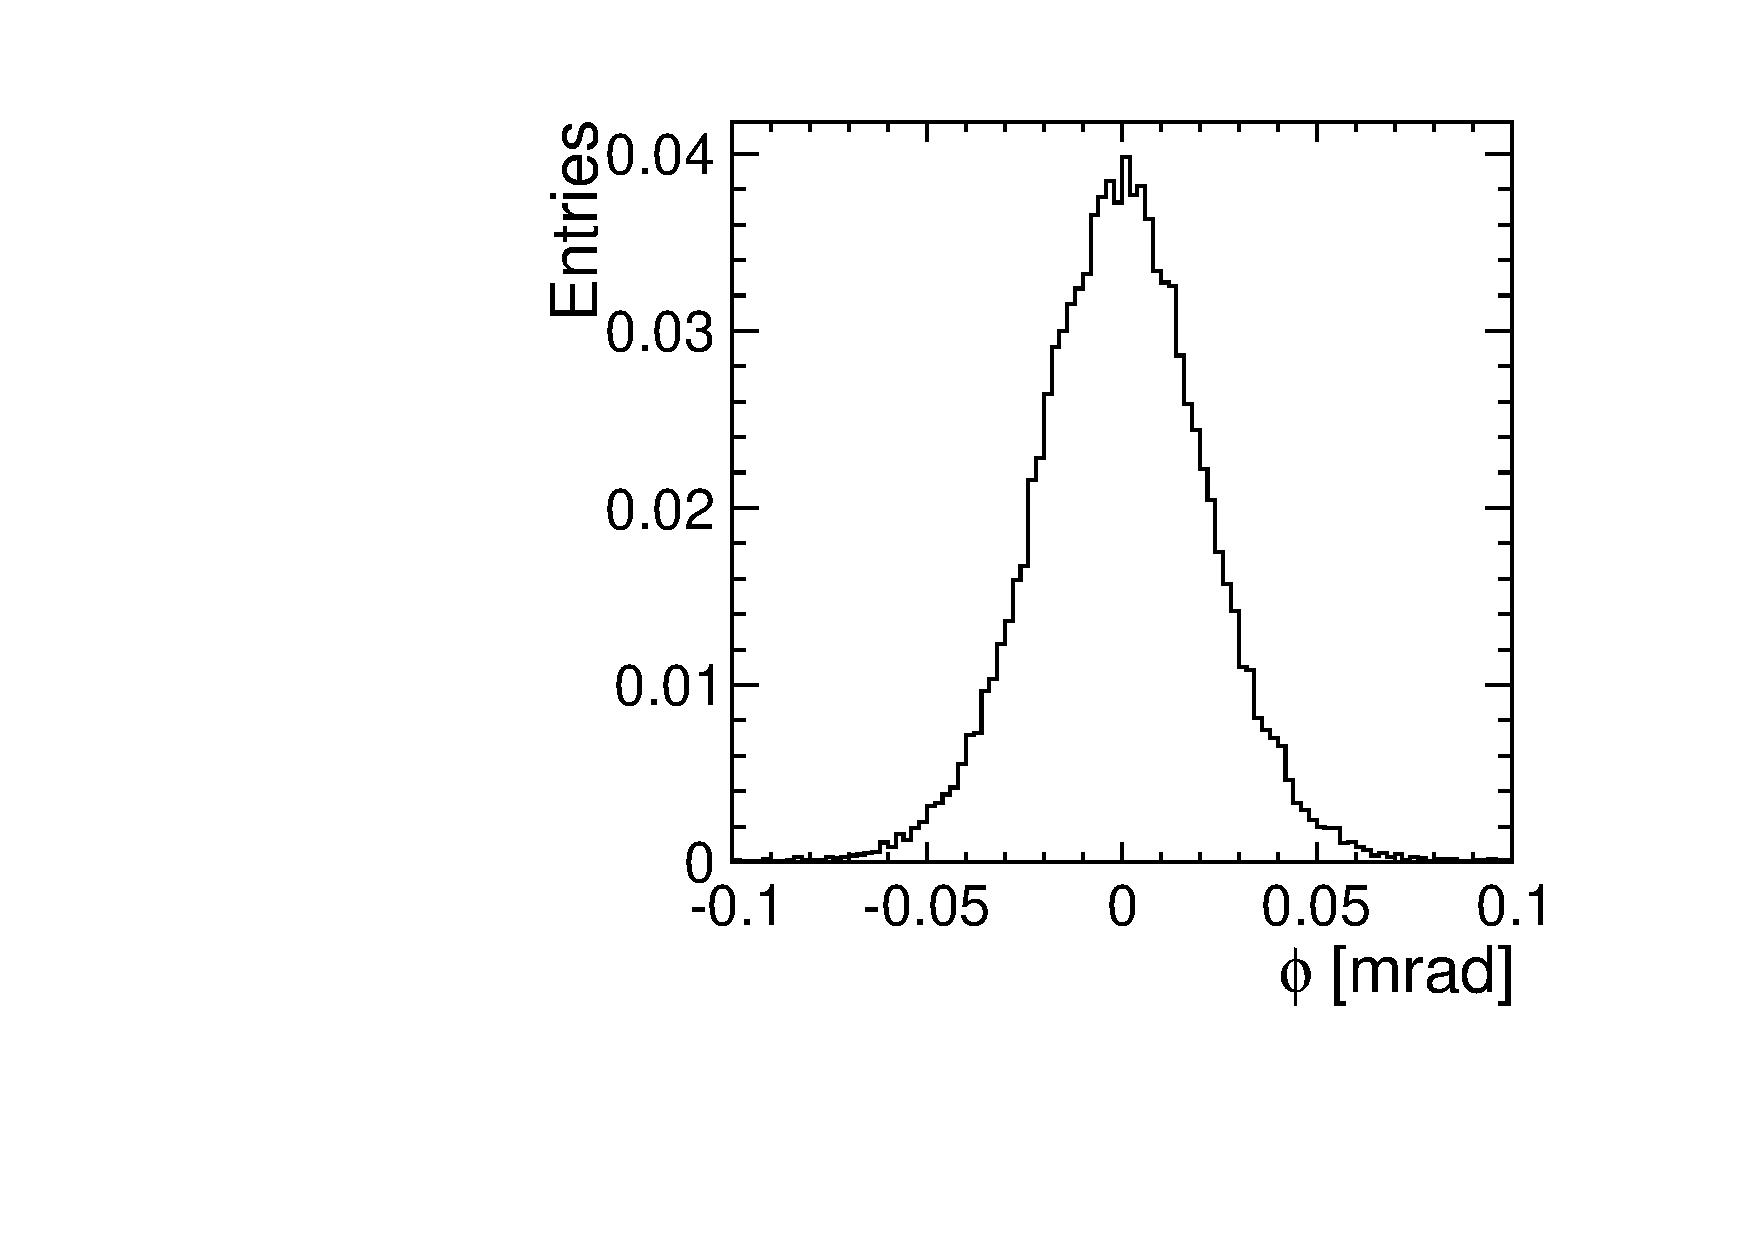
\includegraphics[width=\textwidth]{./figures/Telescope/MC_trackAnglePhi_planes_302_100.pdf}
    \caption{}
  \end{subfigure}\hfill
  \begin{subfigure}[b]{0.45\textwidth}
    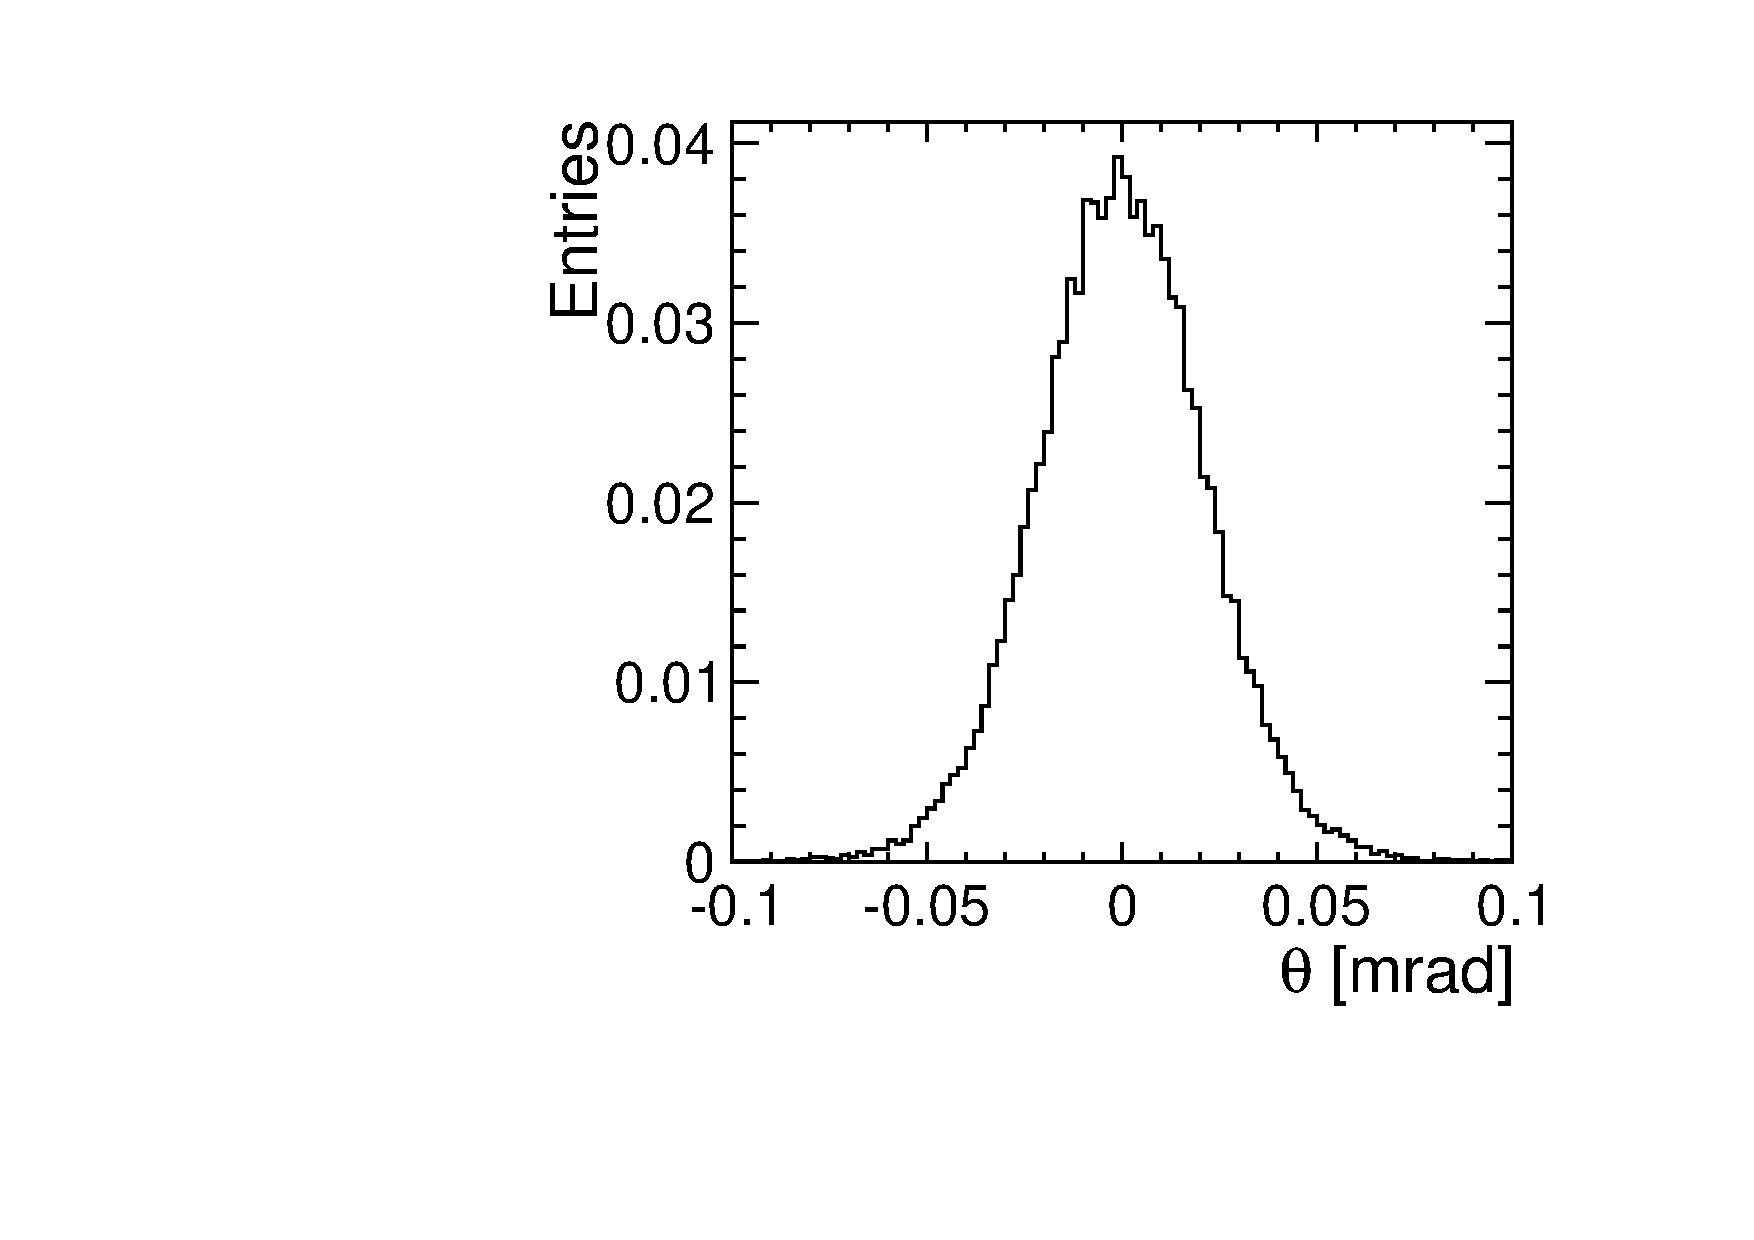
\includegraphics[width=\textwidth]{./figures/Telescope/MC_trackAngleTheta_planes_302_100.pdf}
    \caption{}
  \end{subfigure}
  \caption{Beam angular distribution in \textsc{Geant4} simulations
(comparing the global positions on the second telescope plane and on
the DUT).}
  \label{fig:MCbeamAngleDistr}
\end{figure}
